\newpage
\chapter{Interfacing a component code with OASIS3-MCT}
\label{sec_modelinterfacing}

At run-time, OASIS3-MCT performs parallel exchange of coupling data between parallel
components and sub-components and allows remapping (interpolation), time integration or accumulation and other transformations of these coupling fields. 

This chapter describes how to adapt the component codes to couple them through OASIS3-MCT. 

OASIS3-MCT supports coupling exchanges between parallel
components and sub-components deployed in diverse
configurations; the different possibilities and how to use
the OASIS3-MCT library accordingly are described in section
\ref{sec_deploy}. 
The OASIS3-MCT Application Programming Interface (API) includes different classes of modules or routines that are described in details in section \ref{API}.
Finally, in section \ref{subsubsec_Algoritms}, different coupling
algorithms are illustrated and details on how to reproduce them with
OASIS3-MCT are provided, together with more information on the {\tt LAG} and {\tt
  SEQ} indices.

\section{Configurations of components supported}
\label{sec_deploy}

Since OASIS3-MCT\_3.0, coupling exchanges between components and
sub-components deployed in a much larger diversity of configurations
are now supported. This is illustrated on figure
\ref{Fig_coupling_layouts_a} and how to use the OASIS3-MCT library
accordingly is detailed on figure \ref{Fig_coupling_layouts_b}. All
OASIS3-MCT API routines are also described in details in section
\ref{API}. 

We call here an ``executable'' a compiled code
  forming a part of or the whole coupled system (started with the
  mpirun or mpiexec command). A ``component'' is the ensemble of
  processes, or tasks, within the coupled system calling {\tt oasis\_init\_comp}
  with the same {\tt comp\_name} argument (see section
  \ref{init_comp}). A ``sub-component'' is the subset of tasks within a
  component sending or receiving coupling fields on a specific grid;
  of course, a component may have only one sub-component
  that gathers all its tasks.

Practical examples of how to use the OASIS3-MCT library are also given in {\tt examples/} {\tt tutorial} and {\tt examples/test\_1bin\_ocnice} (see sections \ref{subsec_tutorial} and \ref{subsec_1bin_ocnice}). 

Since OASIS3-MCT\_3.0, it is possible to (the text between [ and ] refers to figure \ref{Fig_coupling_layouts_a}) :

\begin{figure}
  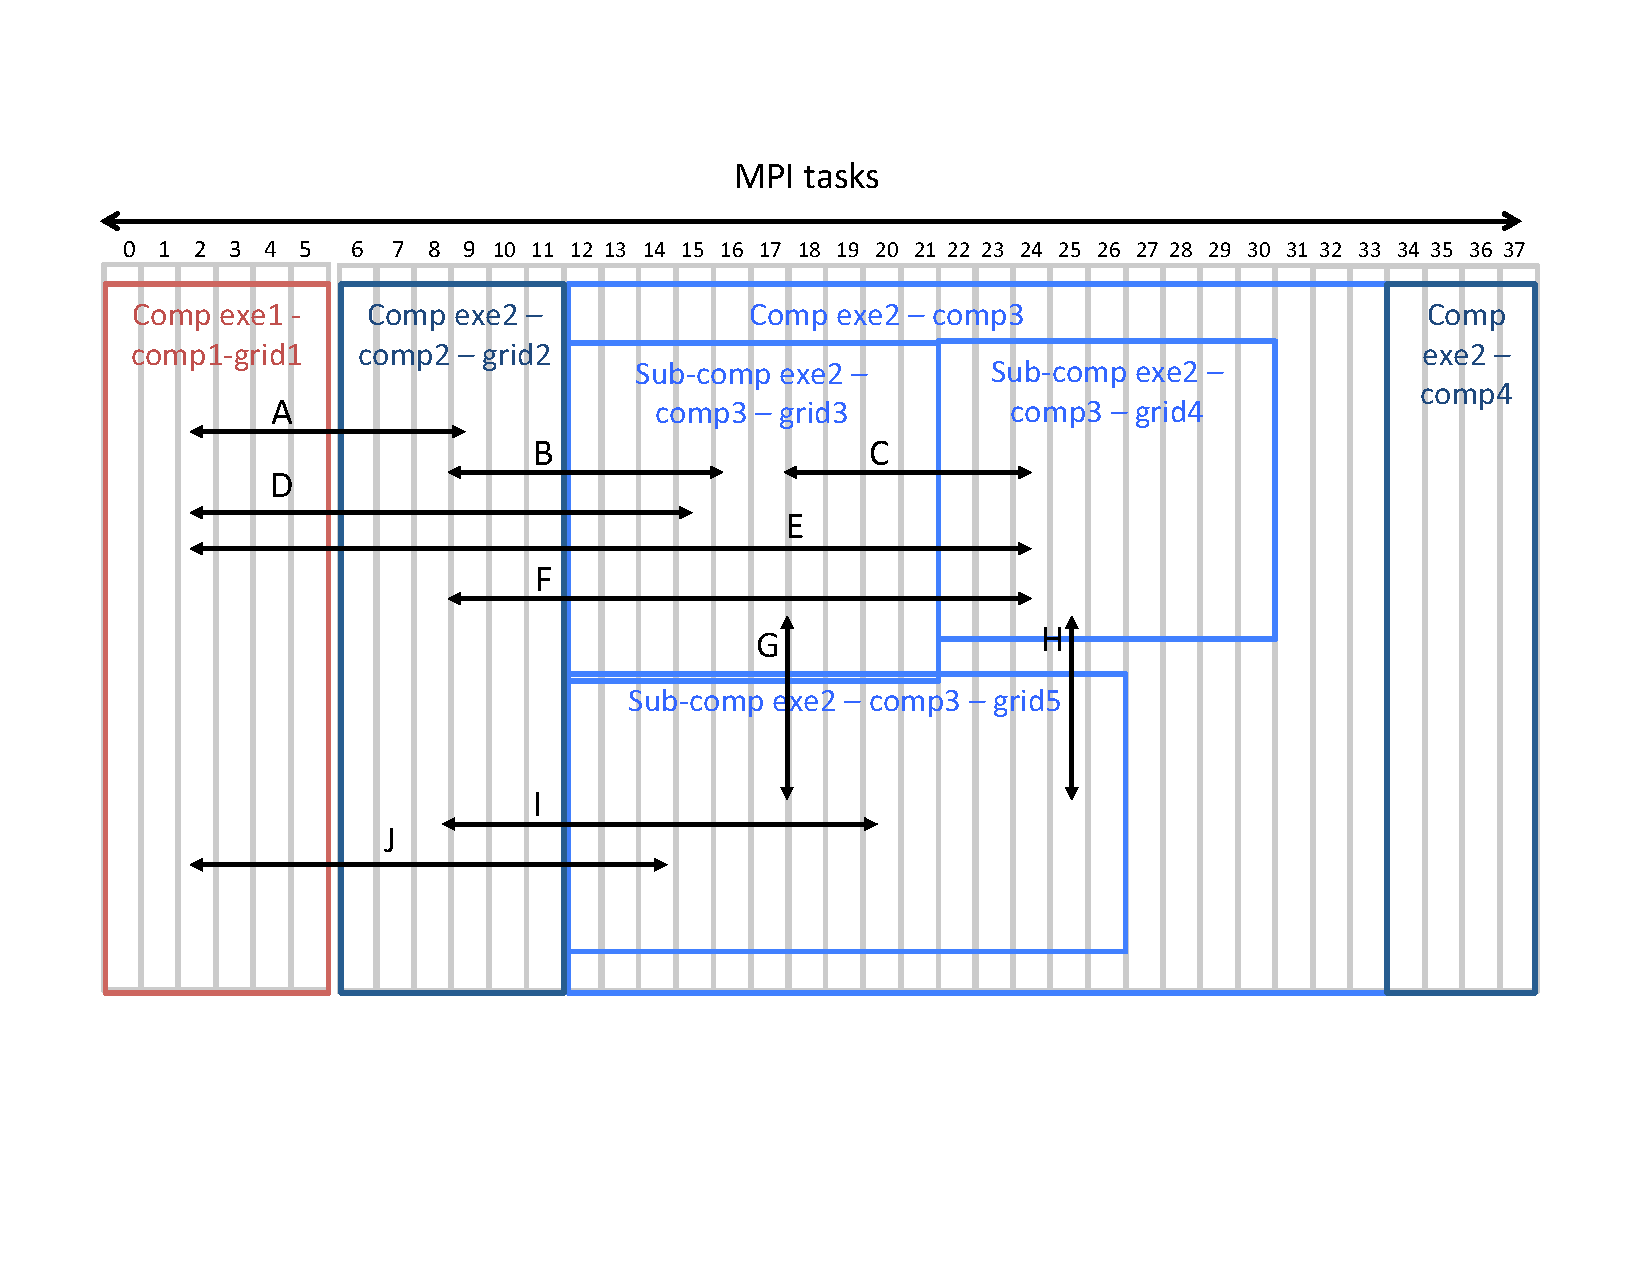
\includegraphics[scale=.6]{figures/coupling_layouts_a}
  \caption{The different configuration of components supported by OASIS3-MCT\_3.0. Two executables {\tt exe1} and {\tt exe2} are running concurrently on separate sets of MPI tasks (0-5 for {\tt exe1} and 6-37 for {\tt exe2}). Executable {\tt exe1} includes only one component {\tt comp1} that has coupling fields defined on only one grid {\tt grid1} (decomposed on all its 6 tasks). Executable {\tt exe2} includes 3 components, {\tt comp2}, {\tt comp3}, and {\tt comp4} running concurrently respectively on tasks 6-11, 12-33 and 34-37. Component {\tt comp2} participates in the coupling with fields defined on only one coupling grid {\tt grid2} (decomposed on all its 5 tasks) while {\tt comp4} does not participate at all in the coupling. 
Component {\tt comp3} has 3 sub-components, respectively exchanging
coupling fields defined on {\tt grid3} (tasks 12-21), {\tt grid4}
(tasks 22-30) and {\tt grid5} (tasks 12-26, therefore overlaping with both {\tt
  grid3} and {\tt grid4}); finally, {\tt comp3} has 3 tasks (31-33)
not involved in the coupling. Sub-components exe2-comp3-grid3 and
exe2-comp3-grid5, or sub-components exe2-comp3-grid4 and
exe2-comp3-grid5 are examples of coupling between sub-components running sequentially on overlapping sets of tasks.}
  \label{Fig_coupling_layouts_a}
\end{figure}

\begin{figure}
  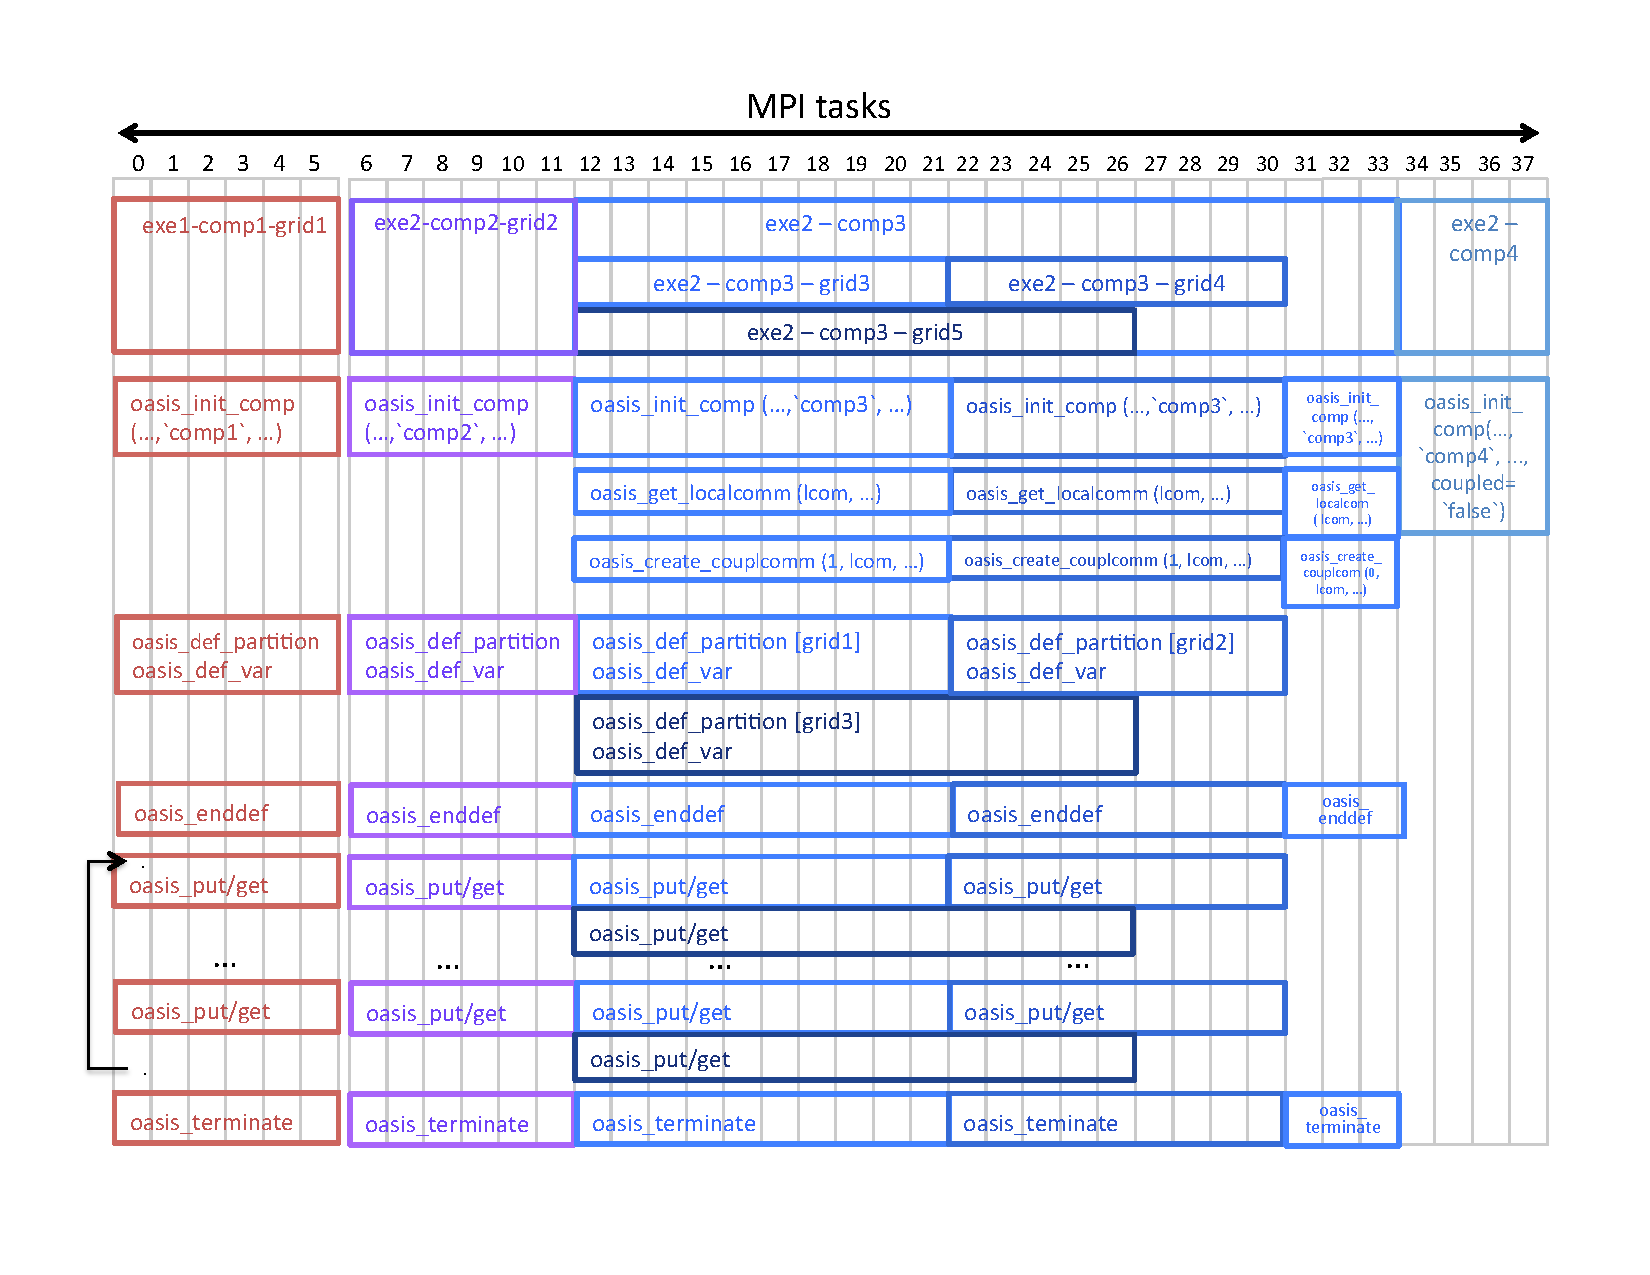
\includegraphics[scale=.6]{figures/coupling_layouts_b}
  \caption{The sequence of OASIS3-MCT calls that have to be implemented in the codes so to allow the configuration of components described on figure \ref{Fig_coupling_layouts_a}.
Each MPI tasks has to call {\tt oasis\_init\_comp} once with the name
of its component as $2^{nd}$ argument. As none of {\tt comp4} tasks is
participating to the coupling, {\tt comp4} tasks calls {\tt
  oasis\_init\_comp} with {\tt coupled=.false.”} as $4^{th}$ argument
and does not call any other OASIS3-MCT routine. As some of {\tt comp3}
tasks are participating to the coupling, all {\tt comp3} tasks have to
call {\tt oasis\_init\_comp}, {\tt oasis\_get\_localcomm}, {\tt
  oasis\_create\_couplcomm}, {\tt oasis\_enddef} and {\tt
  oasis\_terminate} (these are the only routine to be called by {\tt
  comp3} tasks 31-33 not participating to the coupling). To initialise
the coupling exchanges, the tasks of a sub-component holding a field
decomposed on a specific grid have to call the {\tt
  oasis\_def\_partition} to express the decomposition of the grid,
{\tt oasis\_def\_var} to declare the coupling field and {\tt
  oasis\_enddef}. Finally, the tasks of a sub-component exchanging 
coupling fields have to call {\tt oasis\_put} and {\tt oasis\_get} accordingly.
}
  \label{Fig_coupling_layouts_b}
\end{figure}

\begin{itemize}

\item to implement coupling exchanges between two components or
  sub-components running concurrently on separate sets of tasks within two different executables  (as before) [A, D, E, J];
\item to implement coupling exchanges between two components or
  sub-components running concurrently on separate sets of tasks within one same executable [B, F, I];
\item to implement coupling exchanges within one executable between
  two concurrent sub-components [C] 
\item to implement coupling exchanges within one executable between
  two sub-components running sequentially on overlapping sets of tasks (i.e. a task can be coupled to itself calling both the ``put” and the ``get” of the exchange) [G, H]
\item to have some tasks of a component not participating to the coupling exchanges [tasks 31-33 of {\tt exe2-comp3}]
\item to have all processes of a component not participating to the coupling exchanges [{\tt exe2-comp4}, tasks 34-37]

\end{itemize}

The sequence of OASS3-MCT API routines that have to be called in the different cases is detailed on figure  \ref{Fig_coupling_layouts_b}.  These routines are also described in detail in the next section.

\section{OASIS3-MCT Application Programming Interface (API)}
\label{API}

To interact with the rest of the coupled system, few calls of the
OASIS3-MCT library routines, which sources can be found in {\tt
  oasis3-mct/lib/psmile} directory, have to be implemented in the
component codes. They belong to the following classes:
\begin{enumerate}
\item Module to use (section \ref{subsubsec_Use})
\item Initialisation (section \ref{subsubsec_Initialisation})
\item Partition definition (section \ref{subsubsec_Partition})
\item Grid data file definition (section \ref{subsubsec_griddef})
\item Coupling-I/O field declaration (section
  \ref{subsubsec_Declaration})
\item End of definition phase (section
  \ref{subsubsec_Endofdefinition})
\item Coupling-I/O field sending and receiving (section
  \ref{subsubsec_sendingreceiving})
\item Termination (section \ref{subsubsec_Termination})
\item Optional auxiliary routines (section
  \ref{subsubsec_auxroutines})
\end{enumerate}

\subsection{Module to use in the code}
\label{subsubsec_Use}
% {Use}

To use OASIS3-MCT library, a user needs to add in his code:

\begin{itemize}

\item {\tt USE mod\_oasis}

  or

\item {\tt USE mod\_prism}
 
\end{itemize}

Both use statements are valid but only one needs to be used in a particular component. This single use statement provides all methods required. The methods, datatypes, and capabilities
are identical for both the {\tt mod\_prism} or {\tt mod\_oasis}
interfaces, the only difference being the name of the interface. The
interface in module {\tt mod\_prism} is provided for backwards
compatability with prior versions of OASIS3. Use of module {\tt
  mod\_oasis} is recommended and provides access to a set of updated
routine names that will continue to evolve in the future, always
ensuring backward compatibility.  In the following sections, both the
{\tt mod\_prism} and {\tt mod\_oasis} interface names are defined and
a single description of the interface arguments is provided.

\subsection{Initialisation}
\label{subsubsec_Initialisation}
% {Initialisation}

\subsubsection{Coupling initialisation}
\label{init_comp}

\begin{itemize}

\item {\tt CALL oasis\_init\_comp (compid, comp\_name, ierror, coupled, commworld)}
\item {\tt CALL prism\_init\_comp\_proto (compid, comp\_name, ierror, coupled, commworld)}

  \begin{itemize}
  \item {\tt compid [INTEGER; OUT]}: returned component ID
  \item {\tt comp\_name [CHARACTER; IN]}: component name; maximum length of 80 characters 
  \item {\tt ierror [INTEGER; OUT]}: returned error code
  \item {\tt coupled [LOGICAL, OPTIONAL; IN]}: flag to specify if the calling task is participating or not to the coupling ({\tt .true.} by default). 
  \item {\tt commworld [INTEGER, OPTIONAL; IN]} : optional argument to specify the global communicator gathering the components of the coupled model. 
  If not specified, {\tt MPI\_COMM\_WORLD} will be used as the default communicator to startup. All components of the coupled model must 
  specify the same {\tt commworld} argument.

  \end{itemize}
 
  This routine must called by all tasks of all components whether of not they are involved in the coupling \footnote{The component may also call MPI\_Init explicitly, but if so, has to call it before calling {\tt oasis\_init\_comp}; in this case, the component also has to call MPI\_Finalize explicitly, but only after calling {\tt oasis\_terminate}.}. 

A component is defined as the ensemble of tasks  calling {\tt
  oasis\_init\_comp} with the same {\tt comp} {\tt \_name}
argument. If and only if all tasks of a component are excluded from
the coupling, the logical {\tt coupled} can be set to {\tt .false.}
for this component tasks; in this case, {\tt oasis\_init\_comp} is the
only API routine that needs to be called by the component tasks. If at
least one tasks of a component is participating to the coupling, all
component tasks have to call {\tt oasis\_init\_comp} with {\tt
  coupled=.true.} (by default); in this case, the component tasks not
participating to the coupling will also have to call
{\tt oasis\_get\_localcomm}, {\tt oasis\_create\_couplcomm}, {\tt oasis\_enddef} and {\tt oasis\_terminate}.
\end{itemize}

\subsubsection{Communicator for internal parallelisation}
\label{subsec_MPI1}

\begin{itemize}
\item {\tt CALL oasis\_get\_localcomm (local\_comm, ierror )}
\item {\tt CALL prism\_get\_localcomm\_proto (local\_comm, ierror )}

  \begin{itemize}
  \item {\tt local\_comm [INTEGER; OUT]}: value of local communicator
  \item {\tt ierror [INTEGER; OUT]}: returned error code.
  \end{itemize}

  This routine returns the value of a local communicator gathering
  only the tasks of the component, i.e. the tasks that called {\tt
  oasis\_init\_comp} with the same {\tt comp\_name}
argument.

  This may be needed as all executables of the coupled system are started in a pseudo-MPMD
  mode with MPI1 and therefore share automatically the same MPI\_COMM\_WORLD
  communicator.  Another communicator has to be used for the internal
  parallelisation of each component. OASIS3-MCT creates this local
  communicator {\tt local\_comm} based on the value of the {\tt
    comp\_name} argument in the {\tt oasis\_init\_comp} call.

  Retrieving a local communicator {\tt local\_comm} is also needed if
  {\tt oasis\_create\_couplcomm} is called, as {\tt local\_comm} is an argument of this routine (see below).

  % With CLIM-MPI2, OASIS3 executable spawns the component
  % executables at the beginning of the run; the components keep their
  % internal parallelisation context unchanged with respect to their
  % standalone mode. In this case, calling the
  % prism\_get\_localcomm\_proto routine is useless but if called, the
  % communicator MPI\_COMM\_WORLD will be returned as local
  % communicator.
\end{itemize}

\begin{itemize}
\item {\tt CALL oasis\_create\_couplcomm(icpl, local\_comm,
    coupl\_comm, kinfo)}
\item {\tt CALL prism\_create\_couplcomm(icpl, local\_comm,
    coupl\_comm, kinfo)}
  \begin{itemize}
  \item {\tt icpl [INTEGER; IN]}: coupling process flag
  \item {\tt local\_comm [INTEGER; IN]}: MPI communicator with all
    processes of the component
  \item {\tt coupl\_comm [INTEGER; OUT]}: returned MPI communicator
    gathering only component processes participating in the coupling
  \item {\tt kinfo [INTEGER; OUT; OPTIONAL]}: returned error code
  \end{itemize}

  This routine creates a coupling communicator for a subset of
  processes. It is mandatory to call this routine if only a subset of
  the component processes participate in the coupling (e.g. {\tt comp3} in figure
    \ref{Fig_coupling_layouts_b}); in that case, the processes
    involved in the coupling have to call it with icpl=1 while the
    other have to call it with icpl = MPI UNDEFINED. Argument
    local\_comm is the MPI communicator associated with all processes
    of the component returned by oasis\_get\_localcomm. The new coupling 
    communicator is returned in coupl\_comm.

\end{itemize}
If this communicator already exists in the code, the component should
simply provide it to OASIS3-MCT with:

\begin{itemize}
\item {\tt CALL oasis\_set\_couplcomm(coupl\_comm, kinfo)}
\item {\tt CALL prism\_set\_couplcomm(coupl\_comm, kinfo)}
  \begin{itemize}
  \item {\tt coupl\_comm [INTEGER; IN]}: MPI communicator gathering
    only component processes participating in the coupling
  \item {\tt kinfo [INTEGER; OUT; OPTIONAL]}: returned error code
  \end{itemize}

  This routine allows to provide a local coupling communicator to
  OASIS3-MCT, given that it already exists in the code. The value of
  {\tt coupl\_comm} must be the value of this local coupling
  communicator for the processes participating to the coupling and it
  must be {\tt MPI\_COMM\_NULL} for processes not involved in the
  coupling.
\end{itemize}

\subsection{Partition definition}
\label{subsubsec_Partition}

The coupling fields sent or received by a component are usually
scattered among the different component processes. With OASIS3-MCT,
all processes exchanging coupling data have to express in a global index space the local
partitioning of the different grids onto which the data is expressed (see \ref{subsubsec_griddef} for the grid definition).
The processes not implied in the
coupling do not have to call this routine (for backward compatibility with OASIS3-MCT\_2.0,
they may still call it describing a null partition, i.e. with {\tt ig\_paral(:)=0}).

\begin{itemize}

  \vspace{0.2cm}
\item {\tt CALL oasis\_def\_partition (il\_part\_id, ig\_paral,
    ierror, isize, name)} or
\item {\tt CALL prism\_def\_partition\_proto (il\_part\_id, ig\_paral,
    ierror, isize, name)}

  \begin{itemize}
  \item {\tt il\_part\_id [INTEGER; OUT]}: partition ID
  \item {\tt ig\_paral [INTEGER, DIMENSION(:), IN]}: vector of
    integers describing the local grid partition in the global index space;
    has a different expression depending on the type of the partition;
    in OASIS3-MCT, 5 types of partition are supported: Serial (no
    partition), Apple, Box, Orange, and Points (see below).
  \item {\tt ierror [INTEGER; OUT]}: returned error code.
  \item {\tt isize [INTEGER, OPTIONAL, IN]}: Optional argument, mandatory
    if the coupling data is exchanged for only a subdomain of the
    global grid; in this case, {\tt isize} must give the total number of grid points.

  \item {\tt name [CHARACTER, OPTIONAL, IN]}: Optional argument associating a name to the partition,
    mandatory if oasis\_def\_partition is called either for a grid
    decomposed not across all the processes of a component or if the related
    oasis\_def\_partition are not
    called in the same order on the different component processes;
    this argument is new since OASIS3-MCT\_3.0 and is linked to the
    greater flexibility in the configuration of components supported
    (see \ref{sec_deploy}); it has a maximum length of 120 characters. 
  \end{itemize}
\end{itemize}

\subsubsection{Serial (no partition)}

This is the choice for a grid entirely supported by only one process . In this case, we have {\tt
  ig\_paral(1:3)}:
\begin{itemize}
\item {\tt ig\_paral(1)} = 0 (indicates a Serial ``partition'')
\item {\tt ig\_paral(2)} = 0
\item {\tt ig\_paral(3)} = the total grid size.
\end{itemize}

\subsubsection{Apple partition}

Each partition is a segment of the global domain, described by its
global offset and its local size. In this case, we have {\tt
  ig\_paral(1:3)}:
\begin{itemize}
\item {\tt ig\_paral(1)} = 1 (indicates an Apple partition)
\item {\tt ig\_paral(2)} = the segment global offset
\item {\tt ig\_paral(3)} = the segment local size
\end{itemize}

Figure \ref{apple_partition} illustrates an Apple partition over 3
processes.
\begin{figure}
  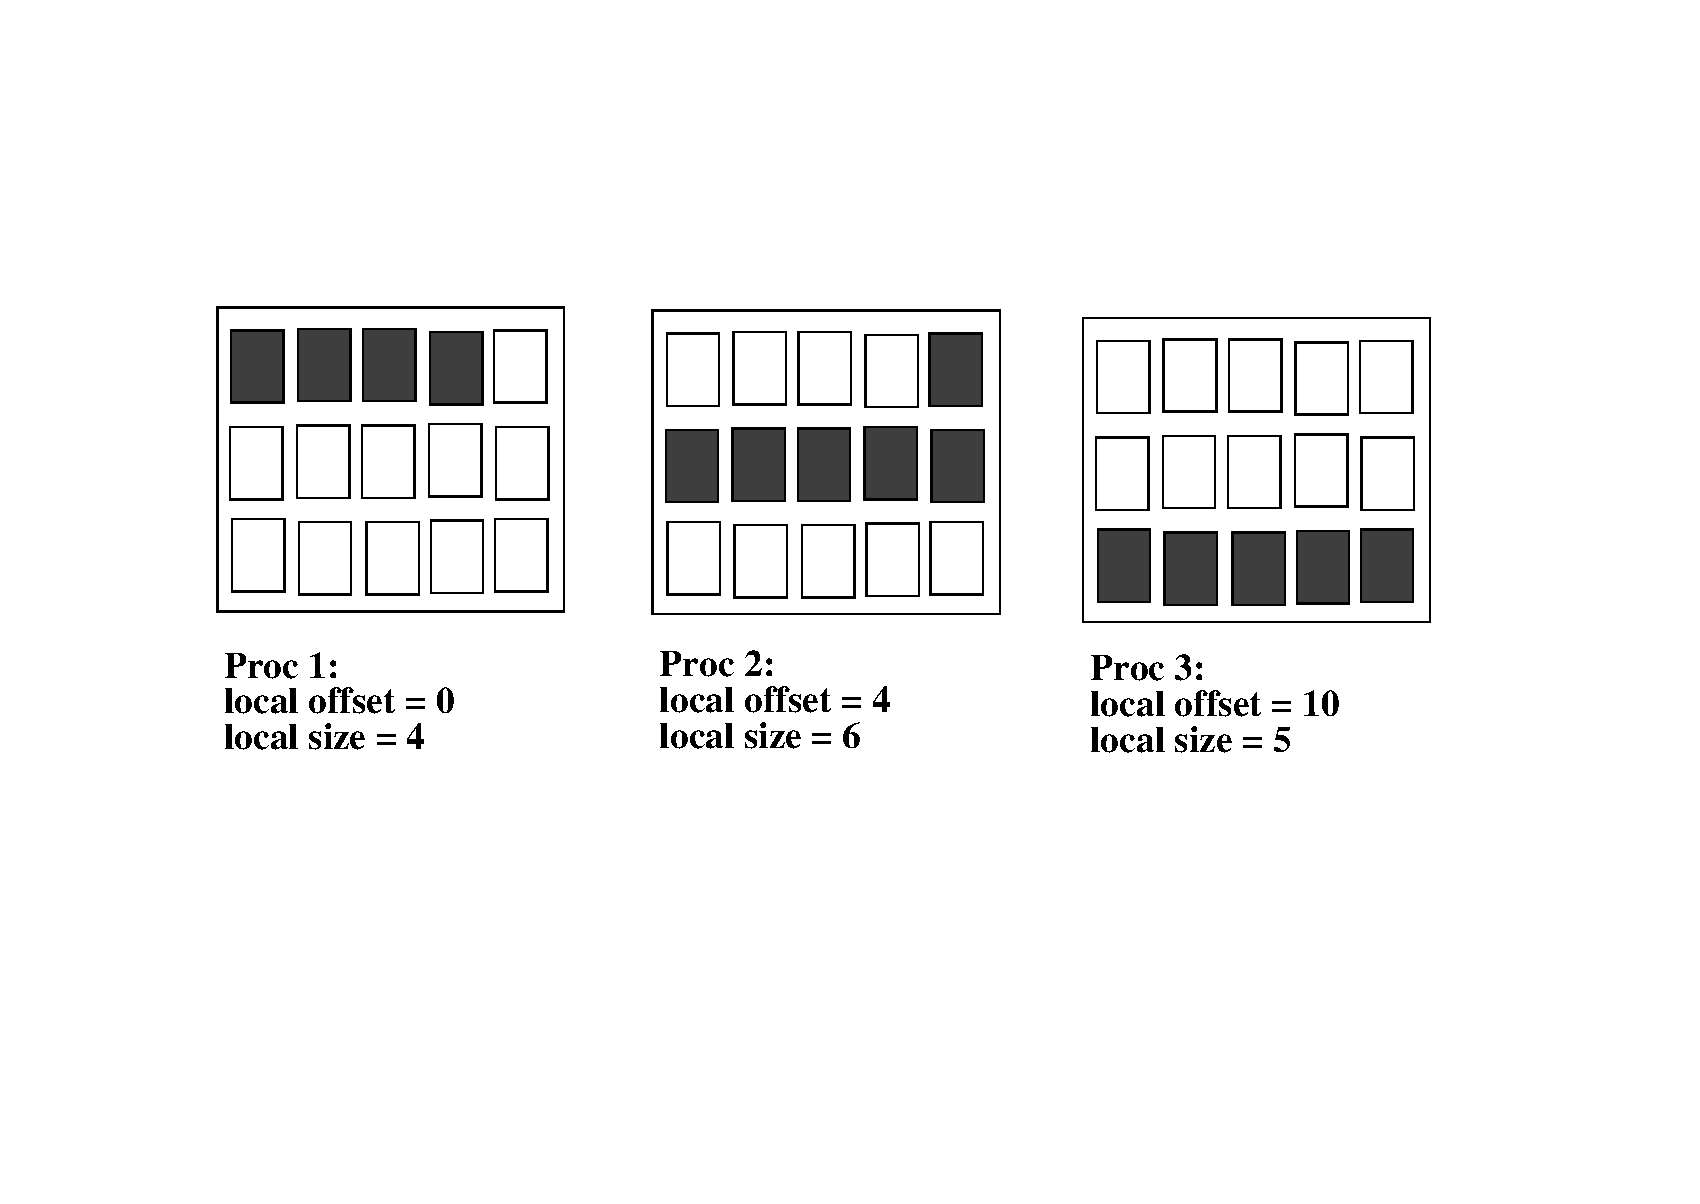
\includegraphics[scale=.6]{figures/apple_new}
  \caption{Apple partition. It is assumed here that the global index starts at
    0 in the upper left corner.}
  \label{apple_partition}
\end{figure}


\subsubsection{Box partition}

Each partition is a rectangular region of the global domain, described
by the global offset of its upper left corner, and its local extents
in the X and Y dimensions. The global extent in the X dimension must
also be given. In this case, we have {\tt ig\_paral(1:5)}:
\begin{itemize}
\item {\tt ig\_paral(1)} = 2 (indicates a Box partition)
\item {\tt ig\_paral(2)} = the upper left corner global offset
\item {\tt ig\_paral(3)} = the local extent in x
\item {\tt ig\_paral(4)} = the local extent in y
\item {\tt ig\_paral(5)} = the global extent in x.
\end{itemize}

Figure \ref{box_partition} illustrates a Box partition over 3
processes.
 
\begin{figure}
  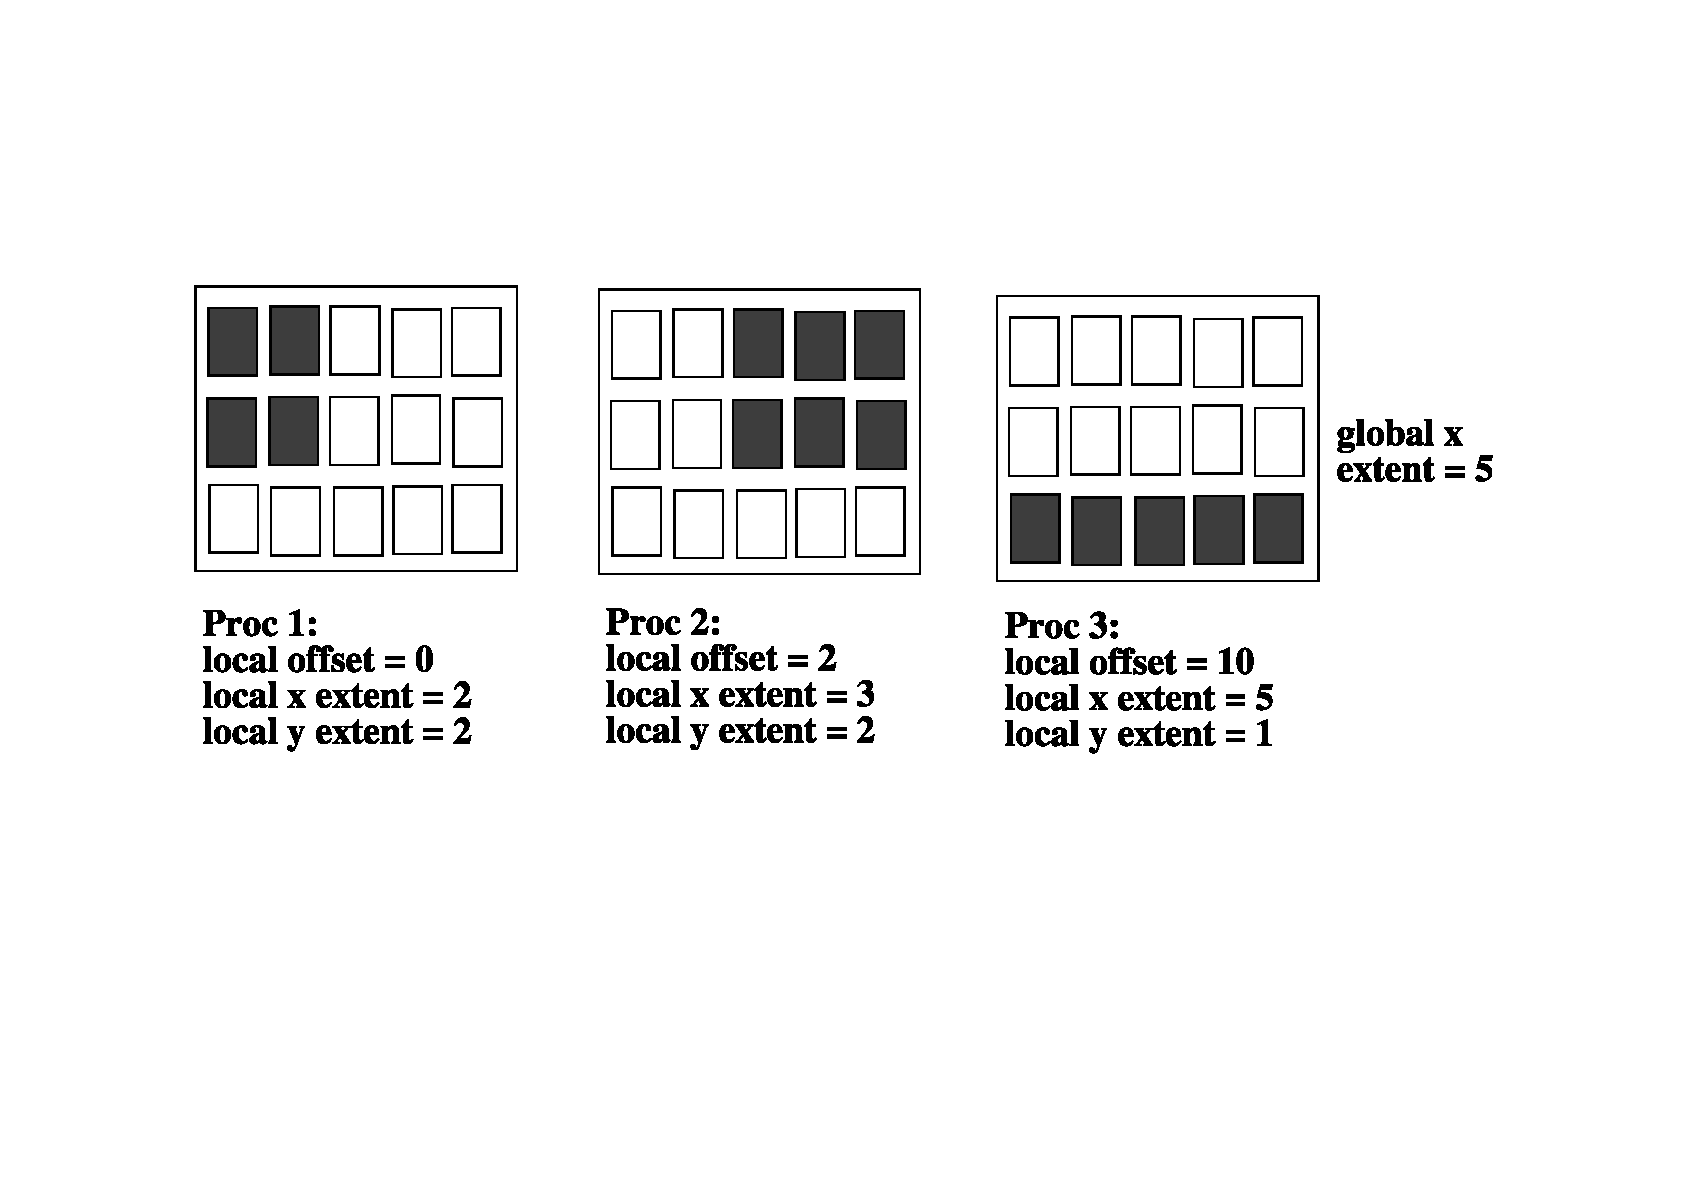
\includegraphics[scale=.6]{figures/box_new}
  \caption{Box partition. It is assumed here that the global index starts at 0
    in the upper left corner.}
  \label{box_partition}
\end{figure}
  
\subsubsection{Orange partition}

Each partition is an ensemble of segments in the global domain. Each
segment is described by its global offset and its local extent.  In
this case, we have {\tt ig\_paral(1:N)} where {\tt N = 2 + 2*number of
  segments}
% \footnote{As for the Box partition, the maximum number of segments
%   is presently 338; it can be increased by modifying the value of
%   {\tt Clim\_MaxSegments}}.

\begin{itemize}
\item {\tt ig\_paral(1)} = 3 (indicates a Orange partition)
\item {\tt ig\_paral(2)} = the total number of segments for the
  partition (limited to 200 presently, see note for ig\_paral(4) for
  Box partition above)
\item {\tt ig\_paral(3)} = the first segment global offset
\item {\tt ig\_paral(4)} = the first segment local extent
\item {\tt ig\_paral(5)} = the second segment global offset
\item {\tt ig\_paral(6)} = the second segment local extent
\item ...
\item {\tt ig\_paral(N-1)} = the last segment global offset
\item {\tt ig\_paral(N)} = the last segment local extent
\end{itemize}

Figure \ref{orange_partition} illustrates an Orange partition with 3
segments for one process. The other process partitions are not
illustrated.

\begin{figure}
  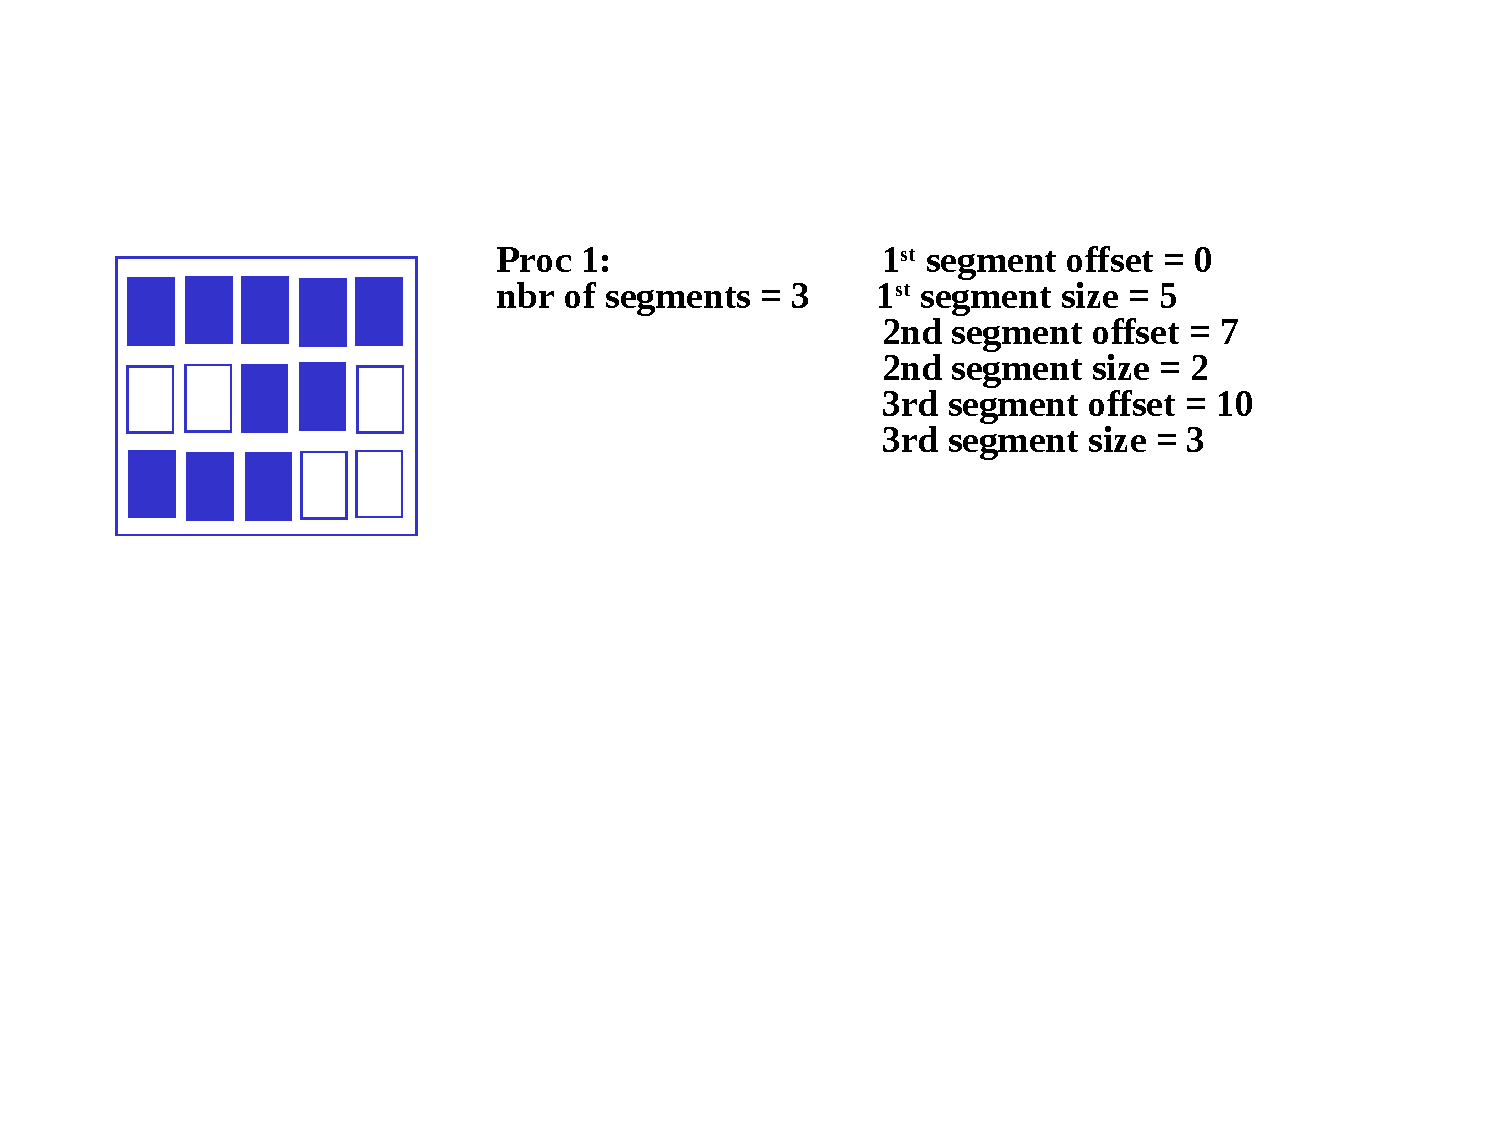
\includegraphics[scale=.6]{figures/orange_new}
  \caption{Orange partition for one process. It is assumed here that
    the global index starts at 0 in the upper left corner.}
  \label{orange_partition}
\end{figure}

\subsubsection{Points partition}

This partition is a list of global indices associated with each
process.  The index naming
is arbitrary but must be consistent between all processes involved
in the partition description.  In
this case, we have {\tt ig\_paral(1:N)} where {\tt N = 2 + number of
  points}
% \footnote{As for the Box partition, the maximum number of segments
%   is presently 338; it can be increased by modifying the value of
%   {\tt Clim\_MaxSegments}}.

\begin{itemize}
\item {\tt ig\_paral(1)} = 4 (indicates a Points partition)
\item {\tt ig\_paral(2)} = number of points in the partition 
\item {\tt ig\_paral(3)} = the first global index
\item {\tt ig\_paral(4)} = the second global index
\item ...
\item {\tt ig\_paral(N)} = the last global index
\end{itemize}

% {Partition definition}
\subsection{Grid data file definition}
\label{subsubsec_griddef}

Grid data files (see section \ref{subsec_griddata}) are required by OASIS3-MCT for specific operations , i.e.  {\em grids.nc} and {\em masks.nc} for
{\tt SCRIPR} (see section \ref{subsec_interp}), and {\em masks.nc} and
{\em areas.nc} for {\tt CONSERV} (see section
\ref{subsec_cooking}). These grid data files can be created by the
user before the run or can be written directly at run time by the components with the following routines.
If a grid data files does not exist, the corresponding routine will create it; if the grid data file exists, the routine can be used to {\bf add} grid definition fields but it will not {\bf overwrite} grid definition fields already existing in the file with the same grid name. 

These routines can be called only by one component process to write the whole grid or by each process holding a part of a grid. In the former case, optional argument {\tt il\_part\_id} is not needed and the arrays (see below) handling the longitudes of the grid points or corners ({\tt lon}, {\tt clon}), the latitudes of the grid points or corners ({\tt lat}, {\tt clat}), the masks ({\tt mask}) and areas ({\tt area}) of the grid cells need to cover the whole grid; in the later case, the {\tt il\_part\_id} returned by {\tt oasis\_def\_partition} needs to be provided as input argument and the arrays need to cover only the local partition of the grid .

\begin{itemize}

\item {\tt CALL oasis\_start\_grids\_writing (flag)} or
\item {\tt CALL prism\_start\_grids\_writing (flag)}
  \begin{itemize}
  \item {\tt flag [INTEGER; OUT]}: always 1 
  \end{itemize} 
Must be called to start the grid writing process. 
  
  \vspace{0.2cm}
\item {\tt CALL oasis\_write\_grid (cgrid, nx\_global, ny\_global, lon, lat, il\_part\_id)}
\item {\tt CALL prism\_write\_grid (cgrid, nx\_global, ny\_global, lon, lat, il\_part\_id)}
        
  \begin{itemize}
  \item {\tt cgrid [CHARACTER; IN]}: grid name prefix (see
    \ref{subsec_namcouplesecond} and \ref{subsec_griddata}); maximum length of 64 characters (4 are usually used for historical reasons)
  \item {\tt nx\_global [INTEGER; IN]} : first dimension of the global grid 
  \item {\tt ny\_global [INTEGER; IN]} : second dimension of the global grid ({\tt =0} if the grid is expressed as a 1D vector) 
  \item {\tt lon [REAL, DIMENSION(nx,ny); IN]} : single or double real array of longitudes covering the whole grid ({\tt nx=nx\_global}, {\tt ny=ny\_global}) or only the local partition (degrees East).
  \item {\tt lat [REAL, DIMENSION(nx,ny); IN]} : single or double real array of latitudes covering the whole grid ({\tt nx=nx\_global}, {\tt ny=ny\_global}) or only the local partition (degrees North)
\item  {\tt il\_part\_id [INTEGER, OPTIONAL; IN]}: partition ID returned by {\tt oasis\_def\_partition}, see \ref{subsubsec_Partition}; needed if each component task holding a part of a decomposed grid writes its own part of the grid.
  \end{itemize}

  Writes the component grid longitudes and latitudes. Longitudes must be
  given in degrees East in the interval -360.0 to 720.0. Latitudes
  must be given in degrees North in the interval -90.0 to 90.0. Note
  that if some grid points overlap, it is recommended to define those
  points with the same number (e.g. 90.0 for both, not 450.0 for one
  and 90.0 for the other) to ensure automatic detection of overlap by
  OASIS3-MCT (which is essential to have a correct conservative
  remapping \texttt{SCRIPR/CONSERV}, see section \ref{subsec_interp}).

  \vspace{0.2cm}
\item {\tt CALL oasis\_write\_corner (cgrid, nx\_global, ny\_global, nc, clon, clat, il\_part\_id))}
\item {\tt CALL prism\_write\_corner (cgrid, nx\_global, ny\_global, nc, clon, clat, il\_part\_id))}

  \begin{itemize}
  \item {\tt cgrid }, {\tt nx\_global }, {\tt ny\_global }, {\tt il\_part\_id }: as for {\tt oasis\_write\_grid}

  \item {\tt nc [INTEGER; IN]} : number of corners per grid cell
    (always 4 in the version)
  \item {\tt clon [REAL, DIMENSION (nx,ny,nc);IN]} : single or double real array of corner
    longitudes covering the whole grid ({\tt nx=nx\_global}, {\tt ny=ny\_global}) or only the local partition (in degrees\_East)
  \item {\tt clat [REAL, DIMENSION (nx,ny,nc);IN]} : single or double real array of corner
    latitudes covering the whole grid ({\tt nx=nx\_global}, {\tt ny=ny\_global}) or only the local partition (in degrees\_North)
  \end{itemize}

  Writes the grid cell corner longitudes and latitudes
  (counterclockwise sense). Longitudes must be given in degrees East
  in the interval -360.0 to 720.0. Latitudes must be given in degrees
  North in the interval -90.0 to 90.0. Note also that cells larger
  than 180.0 degrees in longitude are not supported. Writing of
  corners is optional as corner information is needed only for {\tt
    SCRIPR/CONSERV} (see section \ref{subsec_interp}). If called,
  needs to be called after {\tt oasis/prism\_write\_grid}.

  \vspace{0.2cm}
\item {\tt CALL oasis\_write\_mask (cgrid, nx\_global, ny\_global, mask, il\_part\_id)}
\item {\tt CALL prism\_write\_mask (cgrid, nx\_global, ny\_global, mask, il\_part\_id)}

  \begin{itemize}
  \item {\tt cgrid }, {\tt nx\_global }, {\tt ny\_global }, {\tt il\_part\_id }: as for {\tt oasis\_write\_grid}
  \item {\tt mask [INTEGER, DIMENSION(nx,ny) ;IN]} : mask array covering the whole grid ({\tt nx=nx\_global}, {\tt ny=ny\_global}) or only the local partition (be
    careful about the OASIS historical convention (!): 0 = not masked,
    1 = masked)
  \end{itemize}
  Writes the component grid mask.

  \vspace{0.2cm}
\item {\tt CALL oasis\_write\_area (cgrid, nx\_global, ny\_global, area, il\_part\_id)}
\item {\tt CALL prism\_write\_area (cgrid, nx\_global, ny\_global, area, il\_part\_id)}

  \begin{itemize}
  \item {\tt cgrid }, {\tt nx\_global }, {\tt ny\_global }, {\tt il\_part\_id }: as for {\tt oasis\_write\_grid}
  \item {\tt area [REAL, DIMENSION(nx,ny); IN]} : single or double real array of grid cell
    areas covering the whole grid ({\tt nx=nx\_global}, {\tt ny=ny\_global}) or only the local partition 
  \end{itemize}
  Writes of the component grid cell areas. Needed only for {\tt CONSERV}
  operation (see section \ref{subsec_cooking}).

  \vspace{0.2cm}
\item {\tt CALL prism\_terminate\_grids\_writing()} or
\item {\tt CALL oasis\_terminate\_grids\_writing()}

\end{itemize}

The creation of the different grid data files is effective in the routine
oasis\_enddef.

\subsection{Coupling field declaration}
\label{subsubsec_Declaration}

All processes of a component that send or receive a coupling field, or a part of it, needs to declare the coupling field.
 
Processes not implied in the
coupling do not have to call this routine at all (for backward
compatibility with OASIS3-MCT\_2.0, they may still call it with any {\tt name} and {\tt il\_part\_id}).

\begin{itemize}

\item {\tt CALL oasis\_def\_var (var\_id, name, il\_part\_id,
    var\_nodims, kinout, \newline var\_actual\_shape, var\_type,
    ierror)} or

\item {\tt CALL prism\_def\_var\_proto(var\_id, name, il\_part\_id,
    var\_nodims, kinout, var\_actual\_shape, var\_type, ierror)}

  \begin{itemize}
  \item {\tt var\_id [INTEGER; OUT]}: coupling field ID.  Note that all 
      coupling fields appearing in the {\it namcouple} must be defined with 
      a call to {\tt oasis\_def\_var}; not doing so would lead to an abort.  
      But all fields defined with a call to {\tt oasis\_def\_var} must not necessarily 
      appear in the {\it namcouple}. If a field does not appear in the {\it namcouple}, 
      the {\tt var\_id} returned by the {\tt oasis\_def\_var} will be equal to -1; 
      the value of the {\tt var\_id} should be tested and the corresponding 
      {\tt oasis\_put} and {\tt oasis\_get} should not be called if {\tt var\_id} 
      equals -1. These constraints are imposed to avoid that a typo in the {\it namcouple}
       would lead to coupling exchanges not corresponding to what the user intends to activate. 
  \item {\tt name [CHARACTER; IN]}: field symbolic name (as in the
    {\it namcouple}); maximum length of 80 characters
  \item {\tt il\_part\_id [INTEGER; IN]}: partition ID returned from {\tt oasis\_def\_partition} (see section
    \ref{subsubsec_Partition})
  \item {\tt var\_nodims [INTEGER, DIMENSION(2); IN]}: var\_nodims(1)
    is not used anymore in OASIS3-MCT so its value can be anything but
    it is still part of the oasis\_def\_var arguments; var\_nodims(2) is the number
    of fields in a bundle (this will be 1 for unbundled fields or greater
    than 1 for fields that are bundled).  
  \item {\tt kinout [INTEGER; IN]}: {\tt OASIS\_In} or {\tt PRISM\_In}
    (i.e. = 21) for fields received by the component; {\tt OASIS\_Out},
    {\tt PRISM\_Out} (i.e. = 20) for fields sent by the component
    \footnote{Parameters OASIS\_In, PRISM\_In, OASIS\_Out, PRISM\_Out
      are defined in
      oasis3-mct/lib/psmile/src/mod\_oasis\_parameters.F90}.
  \item {\tt var\_actual\_shape [INTEGER, DIMENSION(:), IN]}:
    not used anymore; vector of integers of any length (for simplicity
    we advise to pass a vector of length 1)
  \item {\tt var\_type [INTEGER; IN]}: type of coupling field array;
    put {\tt OASIS\_Real} or {\tt PRISM\_Real} (i.e. = 4) for single
    or double precision real arrays.  All coupling data is treated as
    double precision in the coupling layer, but conversion to or from
    single precision data is supported in the interface.
  \item {\tt ierror [INTEGER; OUT]}: returned error code.
  \end{itemize}
\end{itemize}
% {coupling field declaration}

\subsection{End of definition phase}
\label{subsubsec_Endofdefinition}
All processes of components at least partly involved in the coupling (e.g. {\tt comp3} in figure
    \ref{Fig_coupling_layouts_b}) have to close the definition phase. Different configurations of components and corresponding use of {\tt oasis\_enddef} are described in section \ref{sec_deploy} and on figures \ref{Fig_coupling_layouts_a} and \ref{Fig_coupling_layouts_b}.
\begin{itemize}
\item {\tt CALL oasis\_enddef (ierror)}
\item {\tt CALL prism\_enddef\_proto(ierror)}
  \begin{itemize}
  \item ierror [INTEGER; OUT]: returned error code.
  \end{itemize}
\end{itemize}

% {End of definition phase}

\subsection{Sending ``put'' and receiving ``get'' actions}
\label{subsubsec_sendingreceiving}

This section describes how to send (put) and receive (get) fields through
the coupling interface.  This interface supports several ranks and
types of coupling fields.  First, the fields passed into the interface can be 
4 byte or 8 byte reals. The field decomposition must be 
consistent with the decomposition defined in the grid partition (see \ref{subsubsec_Partition})\footnote{But the decomposition of each field can be either one
dimensional or two dimensional and does not
have to match the rank of the grid partition.}  Third, the fields
can be bundled, i.e. have an extra (non-spatial) dimension like for a field covering different ice categories.  The bundled dimension is always the last dimension in any
field passed into the get and put routines.  And the size of the bundle dimension
must match the value defined for the variable in var\_nodims(2) in the
{\tt oasis\_def\_var} interface (see section \ref{subsubsec_Declaration}).

So in general, the fields passed into the get and put interface can have rank
1, 2, or 3 and include the following possible options where fld can be a 4
byte or 8 byte real array.

\begin{itemize}
\item 1D, fld(:) = an single, unbundled field of decomposition rank 1.
\item 2D, fld(:,:) = a single, unbundled field of decomposition rank 2.
\item 1D bundled, fld(:,:) = a bundled set of fields of decomposition rank 1.
  The size of the second dimension must equal the number of fields in the 
  bundle, defined by var\_nodims(2) in the {\tt oasis\_def\_var} interface.
\item 2D bundled, fld(:,:,:) = a bundled set of fields of decomposition rank 2.
  The size of the third dimension must equal the number of fields in the 
  bundle, defined by var\_nodims(2) in the {\tt oasis\_def\_var} interface.
\end{itemize}

%With bundled fields, it is important that the number of fields in the bundle match
%in the two models being coupled.  This requires that the var\_nodims(2) values
%in the send and receive model match the bundle dimension of that bundled coupling field.
Different bundled fields
can have different numbers of fields, but for a given bundled field, the
number of fields must match on the send and receive side.  This is explicitly
checked within the coupling layer and will lead to an abort if not done correctly.
It is possible to define a 1D bundled or 2D bundled field  with a bundle dimension of 1, i.e. for a bundle that contains only one single field.

Finally, the bundled field option can be used to
bundle together multi-level variables, multiple related fields, and other types
of fields.  The fields must share a common partition and common namcouple settings (e.g. interpolation)
to be bundled.  While this is a useful feature for multi-level fields, {\bf this does not mean
that 3D interpolation is supported}.
Each field in the bundle is
treated internally as a separate field in the coupling layer without
any information about the relationship between the fields in the bundle.  In fact,
the bundled field variables are internally renamed and a field number is appended
to the variable name to keep track of the distinct fields in the bundle.  That
updated variable name will appear in restart and output files.


\subsubsection{Sending a coupling (or I/O) field or writing a coupling restart file}
\label{prismput}

In the component time step loop, each process sends its part of the
coupling (or I/O) field.

\begin{itemize}
\item {\tt CALL oasis\_put (var\_id, date, fld1, info, fld2, fld3,
    fld4, fld5, write\_restart)}
\item {\tt CALL prism\_put\_proto(var\_id, date, fld1, info, fld2,
    fld3, fld4, fld5, write\_restart)}
  \begin{itemize}
  \item {\tt var\_id [INTEGER; IN]}: field ID (returned from corresponding {\tt
      oasis\_def\_var}, see section \ref{subsubsec_Declaration})
  \item {\tt date [INTEGER; IN]}: number of seconds (or any other time
    units as long as the same are used in all components and in the {\it
      namcouple}) at the time of the call (by convention at the
    beginning of the timestep)
  \item {\tt fld1 [REAL, IN]}: coupling (or I/O) field array; can be
    1D, 2D, bundled 1D, or bundled 2D, see baove. 
  \item {\tt info [INTEGER; OUT]}: returned info code:
    \begin{itemize}
    \item {\tt OASIS\_Sent} (=4) if the field was sent to another component
    \item {\tt OASIS\_LocTrans} (=5) if the field was only used in a time
      transformation (not sent, not output)
    \item {\tt OASIS\_ToRest} (=6) if the field was written to a restart
      file only
    \item {\tt OASIS\_Output} (=7) if the field was written to an output
      file only
    \item {\tt OASIS\_SentOut} (=8) if the field was both written to an
      output file and sent to another component 
    \item {\tt OASIS\_ToRestOut} (=9) if the field was written both to a
      restart file and to an output file.
    \item {\tt OASIS\_WaitGroup} (=14) if the field was not sent because it is part of a group.
    It will be sent only when the {\tt oasis\_put} of the last field in the group will be called; however, the field is buffered and therefore the field array can be modified in the component code when returning from the oasis\_put call.
    \item {\tt OASIS\_Ok} (=0) otherwise and no error occurred.
    \end{itemize}
  \item {\tt fld2 [REAL, IN, OPTIONAL]}: optional $2^{nd}$ coupling
    field array; can be 1D, 2D, bundled 1D, or bundled 2D.  Rank and size
    must match {\tt fld1}.
  \item {\tt fld3 [REAL, IN, OPTIONAL]}: optional $3^{rd}$ coupling
    field array; can be 1D, 2D, bundled 1D, or bundled 2D.  Rank and size
    must match {\tt fld1}.
  \item {\tt fld4 [REAL, IN, OPTIONAL]}: optional $4^{th}$ coupling
    field array; can be 1D, 2D, bundled 1D, or bundled 2D.  Rank and size
    must match {\tt fld1}.
  \item {\tt fld5 [REAL, IN, OPTIONAL]}: optional $5^{th}$ coupling
    field array; can be 1D, 2D, bundled 1D, or bundled 2D.  Rank and size
    must match {\tt fld1}.
  \item {\tt write\_restart [LOGICAL, IN, OPTIONAL]}: optional argument to write an 
    intermediate restart file associated with the variable {\tt
      var\_id} at the current timestep (see below).
  \end{itemize}
\end{itemize}

To ensure a proper use of the {\tt oasis\_put}, one has to take care
of the following aspects:

\begin{itemize}

\item A $2^{nd}$, $3^{rd}$, $4^{th}$ and $5^{th}$ source field can be
  passed as optional arguments. If so, the $2^{nd}$, $3^{rd}$,
  $4^{th}$ and $5^{th}$ set of weights present in the remapping file
  will be applied, respectively (see section \ref{subsec_mapdata} for
  the remapping file format). This will be used for example for the {\tt
    SCRIPR/BICUBIC} remapping for which a $1^{st}$, $2^{nd}$,
  $3^{rd}$, $4^{th}$ set of weights should be respectively applied to
  the field value, its gradient in the first dimension, its gradient
  in the second dimension, and its cross-gradient. Bicubic and higher order
  remapping are therefore supported given that the higher order fields
  are provided at each time step as {\tt oasis\_put} arguments. Note
  that if {\tt fld3}, or {\tt fld4}, or {\tt fld5} are passed, {\tt fld2}, or {\tt fld3} and 
  {\tt fld2}, or {\tt fld4} and {\tt fld3} and {\tt fld2} must also be passed respectively.
  
\item {\bf Note that from OASIS3-MCT\_4.0 onwards, 
the number of weights in the remapping file and the number of fields in the coupling restart file 
(when such a file is needed) must strictly match the number of source fields passed to the 
oasis\_put .}

%\item Trying to send with {\tt oasis\_put} a field declared with a
%  {\tt oasis\_def\_var} but not defined in the configuration file {\it
%    namcouple} will lead to an abort. In this case, the field ID
%  returned by the {\tt oasis\_def\_var} is equal to -1 and the
%  corresponding {\tt oasis\_put} should not be called.

\item This routine may be called by the component at each timestep. The
  convention for the {\tt date} argument is to indicate the time at
  the beginning of the timestep. The sending is actually performed
  if the time obtained by adding the field lag ({\tt LAG} in the
  {\em namcouple}, if any, with {\tt LAG=0} by default) to the {\tt date} corresponds to a time at which it
  should be activated, given the coupling or I/O period indicated by
  the user in the {\it namcouple} (see section \ref{sec_namcouple}).

\item By convention, the first coupling
  of a run occurs at {\tt date=0} and the final coupling occurs
  at {\tt date = runtime-cpl\_period}, where {\tt runtime} is the total time of
  the run and {\tt cpl\_period} is the coupling period of the field indicated by
  the user in the {\it namcouple} (see section \ref{sec_namcouple}).

\item For a coupling
  field with a positive lag, the coupling restart file (see section
  \ref{subsec_restartdata}) is automatically overwritten by the {\tt
    oasis\_put} when the {\tt date+LAG=runtime}.

  % \item A field will not be sent at all if its coupling (or I/O)
  %   period indicated in the {\it namcouple} is greater than the
  %   total run time.

\item The total run time should match an integer number of coupling
  periods.

\item If a local time transformation is indicated for the field by the
  user in the {\it namcouple} (INSTANT, AVERAGE, ACCUMUL, T\_MIN or
  T\_MAX, see section \ref{sec_transformations}), it is automatically
  performed and the resulting field is finally sent at the coupling or
  I/O frequency.  For non-instant transformations, partially
  transformed fields will be written to the restart file at the end of
  the run for use on the next component startup, when needed.

\item A coupling field sent by a source component can be
  associated with more than one target field and component, if specified
  as so with different entries in the {\it namcouple} configuration
  file. In that case, the source component needs to send the field only
  once and the corresponding data will arrive at multiple targets as
  specified in the {\it namcouple}. Different coupling frequencies and
  transformations are allowed for different coupling exchanges of the
  same field. If coupling restart files are required (either if a {\tt
    LAG} or if a {\tt LOCTRANS} transformation is specified), it is
  mandatory to specify different files for the different fields.

\item Trying to send with {\tt oasis\_put} a field declared with a {\tt
  oasis\_def\_var} but not defined in the configuration file {\it
  namcouple} will lead to an abort. When a field is not defined in the {\it namcouple}, the field ID
returned by the {\tt oasis\_def\_var} is equal to -1 and the
corresponding {\tt oasis\_put} should not be called. 

\item Support to couple multiple fields via a single communication.
This is supported through colon delimited field lists in the namcouple (see \ref{subsubsec_secondEXPORTED}). 
All fields will use the namcouple settings for that entry. In the component
model codes, these fields are still sent ({\bf “put”}) one at a time. Inside
OASIS3-MCT, the fields are stored and a single mapping and send instruction is executed
for all fields. This is useful in cases where multiple fields have the same coupling transformations
and to reduce communication costs by aggregating multiple fields into a single communication.

This option does not put any constraint
on the order of the related {\tt oasis\_put} and {\tt oasis\_get} in the codes.

As they appear in one single entry line, these fields must share the same coupling restart file 
but this restart file may contain other fields.

\item The optional argument, {\tt write\_restart}, in the {\tt oasis\_put} routine is {\bf false} by default. 
If a user sets that argument to true, a restart file will be written for that field {\bf only for that timestep}. The {\tt write\_restart} 
will just save the data that exists at the time of the call, taking into account lags and LOCTRANS operations. In 
cases where multiple fields are coupled as a single operation in the model (indicated via a list of colon delimited 
fields in the {\it namcouple}, see \ref{subsubsec_secondEXPORTED}), users are encouraged to specify 
the {\tt write\_restart} flag on ALL {\tt oasis\_put} calls at a given
time for this set of fields.
Intermediate restarts will be created with a timestamp prepended to
their filename, like TA000003600\_rst4.nc or TC000014400\_rst4.nc. 
A restart file that starts with TA will be a restart file associated
with LOCTRANS operations. A restart 
file that starts with TC will be a restart file associated with
coupling operations. The 9 digit timestamp in 
the filename is the date in seconds at the time of the oasis\_put
call. The restart filename (ie. rst4.nc) 
defined in the namcouple for variables will be used to generate a filename for intermediate restart files.
\end{itemize}

\subsubsection{Receiving a coupling (or I/O) field}

In the component time stepping loop, each process receives its part of the
coupling field.

\begin{itemize}
 
\item {\tt CALL oasis\_get (var\_id, date, fld, info)}
\item {\tt CALL prism\_get\_proto(var\_id, date, fld, info)}
  \begin{itemize}
  \item {\tt var\_id [INTEGER; IN]}: field ID (returned by the corresponding
    {\tt oasis\_def\_var})
  \item {\tt date [INTEGER; IN]}: number of seconds (or any other time
    units as long as the same are used in all components and in the {\it
      namcouple}) at the time of the call (by convention at the
    beginning of the timestep)
  \item {\tt fld [REAL, OUT]}: I/O or coupling field array;  
    can be 1D, 2D, bundled 1D, or bundled 2D.
  \item {\tt info [INTEGER; OUT]}: returned info code:
    \begin{itemize}
    \item OASIS\_Recvd(=3) if the field was received from another
      component
    \item OASIS\_FromRest (=10) if the field was read from a restart
      file only
    \item OASIS\_Input (=11) if the field was read from an input file
      only
    \item OASIS\_RecvOut (=12) if the field was both received from
      another component and written to an output file
    \item OASIS\_FromRestOut (=13) if the field was both read from a
      restart file and written to an output file
    \item OASIS\_Ok (=0) otherwise and no error occurred.
    \end{itemize}
  \end{itemize}
\end{itemize}

To ensure a proper use of the {\tt oasis\_get}, one has to take care of the following aspects:

\begin{itemize}

\item This routine may be called by the component at each timestep. The {\tt
  date} argument is automatically analysed and the receiving action is
actually performed only if {\tt date} corresponds to a time for which
it should be activated, given the period indicated by the user in the
{\it namcouple}. An exchange at the beginning of the run at time=0 is
expected.

\item Trying to receive with {\tt oasis\_get} a field declared with a {\tt
  oasis\_def\_var} but not defined in the configuration file {\it
  namcouple} will lead to an abort. In this case, the field ID
returned by the {\tt oasis\_def\_var} is equal to -1 and the
corresponding {\tt oasis\_get} should not be called. 

\item If a coupling field has a positive lag, the coupling field that
  matches the {\tt oasis\_get} at time=0 will come from a coupling
  restart file written by the last active {\tt oasis\_put} of the
  previous run (see section \ref{subsubsec_Algoritms}). 

\item Support to couple multiple fields via a single communication.
This is supported through colon delimited field lists in the namcouple (see \ref{subsubsec_secondEXPORTED}). 
All fields will use the namcouple settings for that entry. In the component
model codes, these fields are still received (via an {\tt oasis\_get}) one at a time. Inside
OASIS3-MCT, the fields are stored and a single mapping and receive instruction is executed
for all fields. This is useful in cases where multiple fields have the same coupling transformations
and to reduce communication costs by aggregating multiple fields into a single communication. If a
LOCTRANS transformation is needed for these multiple fields, it is necessary to define a restart file
for these multiple fields.
\end{itemize}

\subsection{Termination}
\label{subsubsec_Termination}

\begin{itemize}

\item {\tt CALL oasis\_terminate (ierror)}
\item {\tt CALL prism\_terminate\_proto(ierror)}
  \begin{itemize}
  \item {\tt ierror [INTEGER; OUT]}: returned error code.
  \end{itemize}
All processes of components at least partly involved in the coupling (e.g. {\tt comp3} in figure
    \ref{Fig_coupling_layouts_b}) have to terminate the coupling by
  calling this routine\footnote{If the process called {\tt MPI\_Init}
    (before calling {\tt oasis\_init\_comp}), it must also call {\tt
      MPI\_Finalize} explicitly, but only after calling {\tt
      oasis\_terminate\_proto}.}(normal termination). Different configurations of components and corresponding use of {\tt oasis\_terminate} are described in section \ref{sec_deploy} and on figures \ref{Fig_coupling_layouts_a} and \ref{Fig_coupling_layouts_b}.

  

\end{itemize}

% {Termination}

\subsection{Auxiliary routines}
\label{subsubsec_auxroutines}

The following auxiliary routines are currently available.

\begin{itemize}
\item {\tt CALL oasis\_abort (compid, routine\_name, abort\_message, rcode)}
\item {\tt CALL prism\_abort\_proto(compid, routine\_name,
    abort\_message)}
  \begin{itemize}
  \item {\tt compid [INTEGER; IN]}: component ID (from {\tt
      oasis\_init\_comp})
  \item {\tt routine\_name[CHARACTER*; IN]}: name of calling routine
  \item {\tt abort\_message[CHARACTER*; IN]}: message to be written
    out.
  \item {\tt rcode [INTEGER, OPTIONAL; IN]}: Optional argument. When OASIS 
    aborts, it returns rcode if it is present, else it returns 1
  \end{itemize}

  If a process needs to abort voluntarily, it should do so by calling
  {\tt oasis\_abort}. This will ensure a proper termination of all
  processes in the coupled model communicator. This routine writes the
  name of the calling component, the name of the calling routine, and the
  message to the process debug file (see {\tt \$NLOGPRT} in section
  \ref{subsec_namcouplefirst}).  This routine cannot be called before
  {\tt oasis\_init\_comp}.

  \vspace{0.2cm}
\item {\tt CALL oasis\_get\_debug(debug\_value)}
\item {\tt CALL prism\_get\_debug(debug\_value)}
  \begin{itemize}
  \item {\tt debug\_value [INTEGER; OUT]}: debug value
  \end{itemize}

  This routine may be called at any time to retrieve the current
  OASIS3-MCT internal debug level (see {\tt \$NLOGPRT} in section
  \ref{subsec_namcouplefirst}).  This is useful if the user wants to
  return the original debug value after changing it.

  \vspace{0.2cm}
\item {\tt CALL oasis\_set\_debug(debug\_value)}
\item {\tt CALL prism\_set\_debug(debug\_value)}
  \begin{itemize}
  \item {\tt debug\_value [INTEGER; IN]}: debug value
  \end{itemize}

  This routine may be called at any time to change the debug level in
  OASIS3-MCT.  This method allows users to vary the debug level at
  different points in the component integration.

  \vspace{0.2cm}
\item {\tt CALL oasis\_get\_intercomm(new\_comm, cdnam, kinfo)}
\item {\tt CALL prism\_get\_intercomm(new\_comm, cdnam, kinfo)}
  \begin{itemize}
  \item {\tt new\_comm [INTEGER; OUT]}: mpi intercomm communicator
  \item {\tt cdnam [CHARACTER*; IN]}: other component name (i.e. 2nd argument of  the call to {\tt oasis\_init\_comp} in that component)
  \item {\tt kinfo [INTEGER; OUT; OPTIONAL]}: returned error code
  \end{itemize}

  This routine sets up an MPI intercomm communicator between the root
  processors of two components, the local component and the component
  associated with {\tt cdnam}.  This call is collective across the
  tasks of the two components but other components are not involved.

  \vspace{0.2cm}
\item {\tt CALL oasis\_get\_intracomm(new\_comm, cdnam, kinfo)}
\item {\tt CALL prism\_get\_intracomm(new\_comm, cdnam, kinfo)}
  \begin{itemize}
  \item {\tt new\_comm [INTEGER; OUT]}: mpi intracomm communicator
  \item {\tt cdnam [CHARACTER*; IN]}: other component name (i.e. 2nd argument of  the call to {\tt oasis\_init\_comp} in that component)
  \item {\tt kinfo [INTEGER; OUT; OPTIONAL]}: returned error code
  \end{itemize}

  This routine sets up an MPI intracomm communicator between the root
  processors of two components, the local component and the component
  associated with {\tt cdnam} .  This call is collective across the tasks of
  the two components but other components are not involved.

\item {\tt CALL oasis\_put\_inquire(var\_id, date, kinfo)}
\item {\tt CALL prism\_put\_inquire\_proto(var\_id, date, kinfo)}
  \begin{itemize}
  \item {\tt var\_id [INTEGER; IN]}: field ID (from
  corresponding oasis\_def\_var)
  \item {\tt date [INTEGER; IN]}: as in {\tt oasis\_put}, number of seconds (or any other time
    units as long as the same are used in all components and in the {\it
      namcouple}) in the run at the time of the call
  \item {\tt kinfo [INTEGER; OUT]}: returned info code
    \begin{itemize}
    \item OASIS\_Sent(=4) if the field would be sent to another component
    \item OASIS\_LocTrans (=5) if the field would be only used in a time
      transformation (not sent, not output)
    \item OASIS\_ToRest (=6) if the field would be written to a restart
      file only
    \item OASIS\_Output (=7) if the field would be written to an output
      file only
    \item OASIS\_SentOut (=8) if the field would be both written to an
      output file and sent to another component (directly or via OASIS3
      main process)
    \item OASIS\_ToRestOut (=9) if the field would be written both to a
      restart file and to an output file.
    \item OASIS\_Ok (=0) otherwise and no error occurred.
    \end{itemize}
  \end{itemize}

This routine may be called at any time to
inquire what would happen to the corresponding field (i.e. with same
{\tt var\_id} and at same {\tt date}) below the corresponding {\tt
  oasis\_put}. This maybe useful if, for example, the calculation of
a coupling field is costly and if one wants to compute it only when it is
really sent out.

\item {\tt CALL oasis\_get\_ncpl(var\_id, ncpl, kinfo)}
\item {\tt CALL prism\_get\_ncpl\_proto(var\_id, ncpl, kinfo)}
  \begin{itemize}
  \item {\tt var\_id [INTEGER; IN]}: field ID (from
  corresponding oasis\_def\_var)
  \item {\tt ncpl [INTEGER; OUT]}: number of coupling exchanges in which the field
  is involved (i.e. when a field is sent to multiple targets) 
  \item {\tt kinfo [INTEGER; OUT]}: returned info code
  \end{itemize}

This routine returns the number of coupling exchanges in which the field var\_id is
involved. This number is needed to get the coupling frequencies with the
routine oasis\_get\_freqs, see below.

\item {\tt CALL oasis\_get\_freqs(var\_id, ncpl, cpl\_freqs, kinfo)}
\item {\tt CALL prism\_get\_freqs\_proto(var\_id, ncpl, cpl\_freqs, kinfo)}
  \begin{itemize}
  \item {\tt var\_id [INTEGER; IN]}: field ID (from
  corresponding oasis\_def\_var)
  \item {\tt ncpl [INTEGER; IN]}: number of couplings in which the field
  is involved (i.e. when a field is sent to multiple targets)
   \item {\tt cpl\_freqs [INTEGER; DIMENSION(ncpl); OUT]}: coupling period(s) 
  (in number of seconds) of field var\_id. There is one coupling period for
  each coupling exchange in which the field is involved
  \item {\tt kinfo [INTEGER; OUT]}: returned info code
  \end{itemize}

This routine can be used to retrieve the coupling period(s) of field with
corresponding {\tt var\_id}, as defined in the {\it namcouple}

\end{itemize}

\section{Coupling algorithms - LAG and SEQ concepts}
\label{subsubsec_Algoritms}

Using the OASIS3-MCT coupling library, the user has full flexibility
to reproduce different coupling algorithms. In the components, the
sending and receiving routines, respectively {\tt oasis\_put} and {\tt
  oasis\_get}, can be called at each component timestep, with the
appropriate {\tt date} argument giving the actual time (at the
beginning of the timestep), expressed in number of seconds since the
start of the run, or in any other time units as long as the same are
used in all components and in the {\it namcouple} (see section
\ref{prismput}). This {\tt date} argument is automatically analysed by
the coupling library and depending on the coupling period and the lag chosen by the user for the coupling field in the {\it namcouple} ({\tt LAG}), different coupling algorithms can be reproduced
without modifying the component codes themselves.

With OASIS3-MCT, a sequence index specified for a coupling field in the {\it namcouple} ({\tt SEQ}), 
provides the coupling layer with an ability to detect a deadlock
before it happens and exit.

The LAG and SEQ concept are explained in more detail below and
some examples are provided.

\vspace{-0.3cm}
\subsection{The lag concept}
\label{subsub_lag}

The lag ({\tt LAG}) must be
expressed in the time unit used (that must be the same in the components
and in the {\it namcouple}, see section \ref{prismput}) and can be
positive or negative but should never be larger (in absolute
magnitude) than the coupling period of any field due to problems with
restartability and dead-locking. When a component calls a {\tt
  oasis\_put}, the value of the lag is automatically added to the
value of the {\tt date} argument and the ``put'' is actually performed
when the sum {\tt date+lag} is a coupling time; in the target
component, this ``put'' will match a {\tt oasis\_get} for which the
{\tt date} argument is the same coupling time.
% A positive lag indicates the put will occur sooner than zero lag and
% a negative lag tells the coupler to send the data later than zero
% lag.
So the lag only shifts the time at which the data is sent but not
the time at which the data is received.
 
When the lag is positive, a restart file must be available to initiate
the coupling.  For a field with positive lag, the source
component automatically reads the field in the restart file
during the coupling initialization phase (below the {\tt
  oasis\_enddef}) and send the data to match the {\tt oasis\_get}
performed at time=0 in the target component. The final coupling
data on the source side will then be automatically written to the
restart file for use in the next run\footnote{When there is a lag, the first and last instance of the source field
in the debug netCDF file (EXPOUT fields, see section
\ref{subsec_namcouplesecond}) always correspond respectively to the
field read from and written to the restart file.}.

On the 4 figures in this section, short black arrows correspond to
  {\tt oasis\_put} or {\tt oasis\_get} called in the component
  that do not lead to any ``put" or receiving action; long black
  arrows correspond to {\tt oasis\_put} or {\tt oasis\_get} called in
  the components that do actually lead to a ``put" or ``get''
  action; long red arrows correspond to {\tt oasis\_put} or {\tt
    oasis\_get} called in the component models that lead to a reading
  or writing of the coupling field from or to a coupling restart file.
 
\begin{enumerate}

\item LAG concept first example
 
  A first coupling algorithm, exploiting the LAG concept, is
  illustrated on figure \ref{fig:lag_concept_1}.

  

  \begin{figure}
    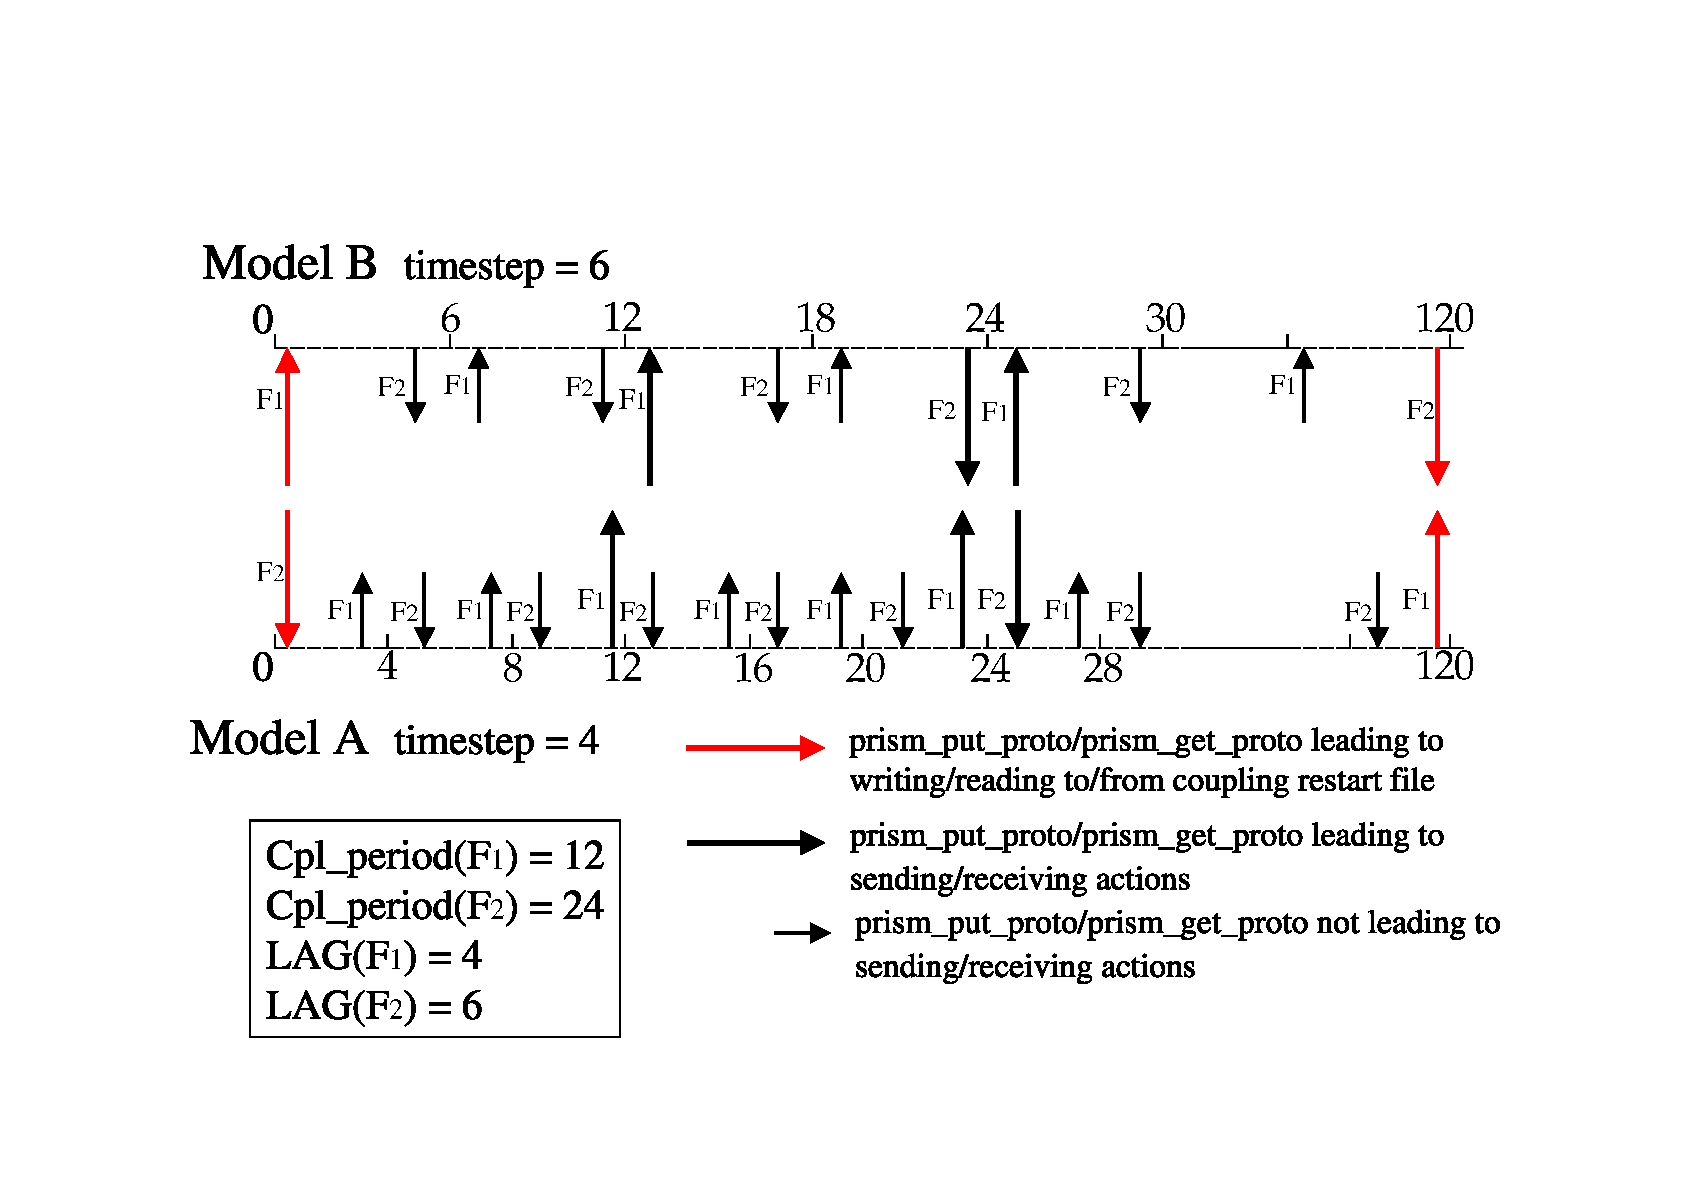
\includegraphics[scale=.6]{figures/fig_lag_concept_1}
    \caption{LAG concept first example}
    \label{fig:lag_concept_1}
  \end{figure}

  During a coupling timestep, model A receives $F_2$ and then sends
  $F_1$; its timestep length is 4. During a coupling timestep, model B
  receives $F_1$ and then sends $F_2$; its timestep length is 6.
  $F_1$ and $F_2$ coupling periods are respectively 12 and 24. If
  $F_1$/$F_2$ ``put" action by model A/B was used at a coupling
  timestep to match the model B/A ``get" action, a deadlock would
  occur as both models would be initially waiting on a ``get"
  action. To prevent this, $F_1$ and $F_2$ produced at the timestep
  before have to be used to match respectively the model B and model A
  ``get" actions.

  This implies that a lag of respectively 4 and 6 seconds must be
  defined for $F_1$ and $F_2$. For $F_1$, the {\tt oasis\_put}
  performed at time 8 and 20 by model A will then lead to ``put"
  actions (as 8 + 4 = 12 and 20 + 4 = 24 which are coupling periods)
  that match the ``get" actions performed by {\tt oasis\_get} called by model B
  at times 12 and 24.  For $F_2$, the {\tt oasis\_put}
  performed at time 18 by model B then leads to a ``put" action (as 18
  + 6 = 24 which is a coupling period) that matches the ``get" action
  performed at time 24 by the {\tt oasis\_get} called by model A.

  At the beginning of the run, as their LAG index is greater than 0,
  the first {\tt oasis\_get} of $F_1$ and $F_2$ will automatically be
  fulfilled with fields read from their respective coupling restart
  files. The user therefore has to create those coupling restart files
  before the first run in the experiment. At the end of the run, $F_1$
  having a lag greater than 0, is automatically written to its
  coupling restart file below the last $F_1$ {\tt oasis\_put} as the
  {\tt date+lag} equals the total run time. The analogue is true for
  $F_2$. These coupling restart fields will automatically be read in at the beginning
  of the next run below the respective {\tt oasis\_get}.

\item LAG concept second example

  A second coupling algorithm exploiting the LAG concept is
  illustrated on figure \ref{fig:lag_concept_2}. During its timestep,
  model A receives $F_2$, sends $F_3$ and then $F_1$; its timestep
  length is 6. During its timestep, model B receives $F_1$, receives
  $F_3$ and then sends $F_2$; its timestep length is also 6.  $F_1$,
  $F_2$ and $F_3$ coupling periods are both supposed to be equal to
  12.
 
  \begin{figure}
    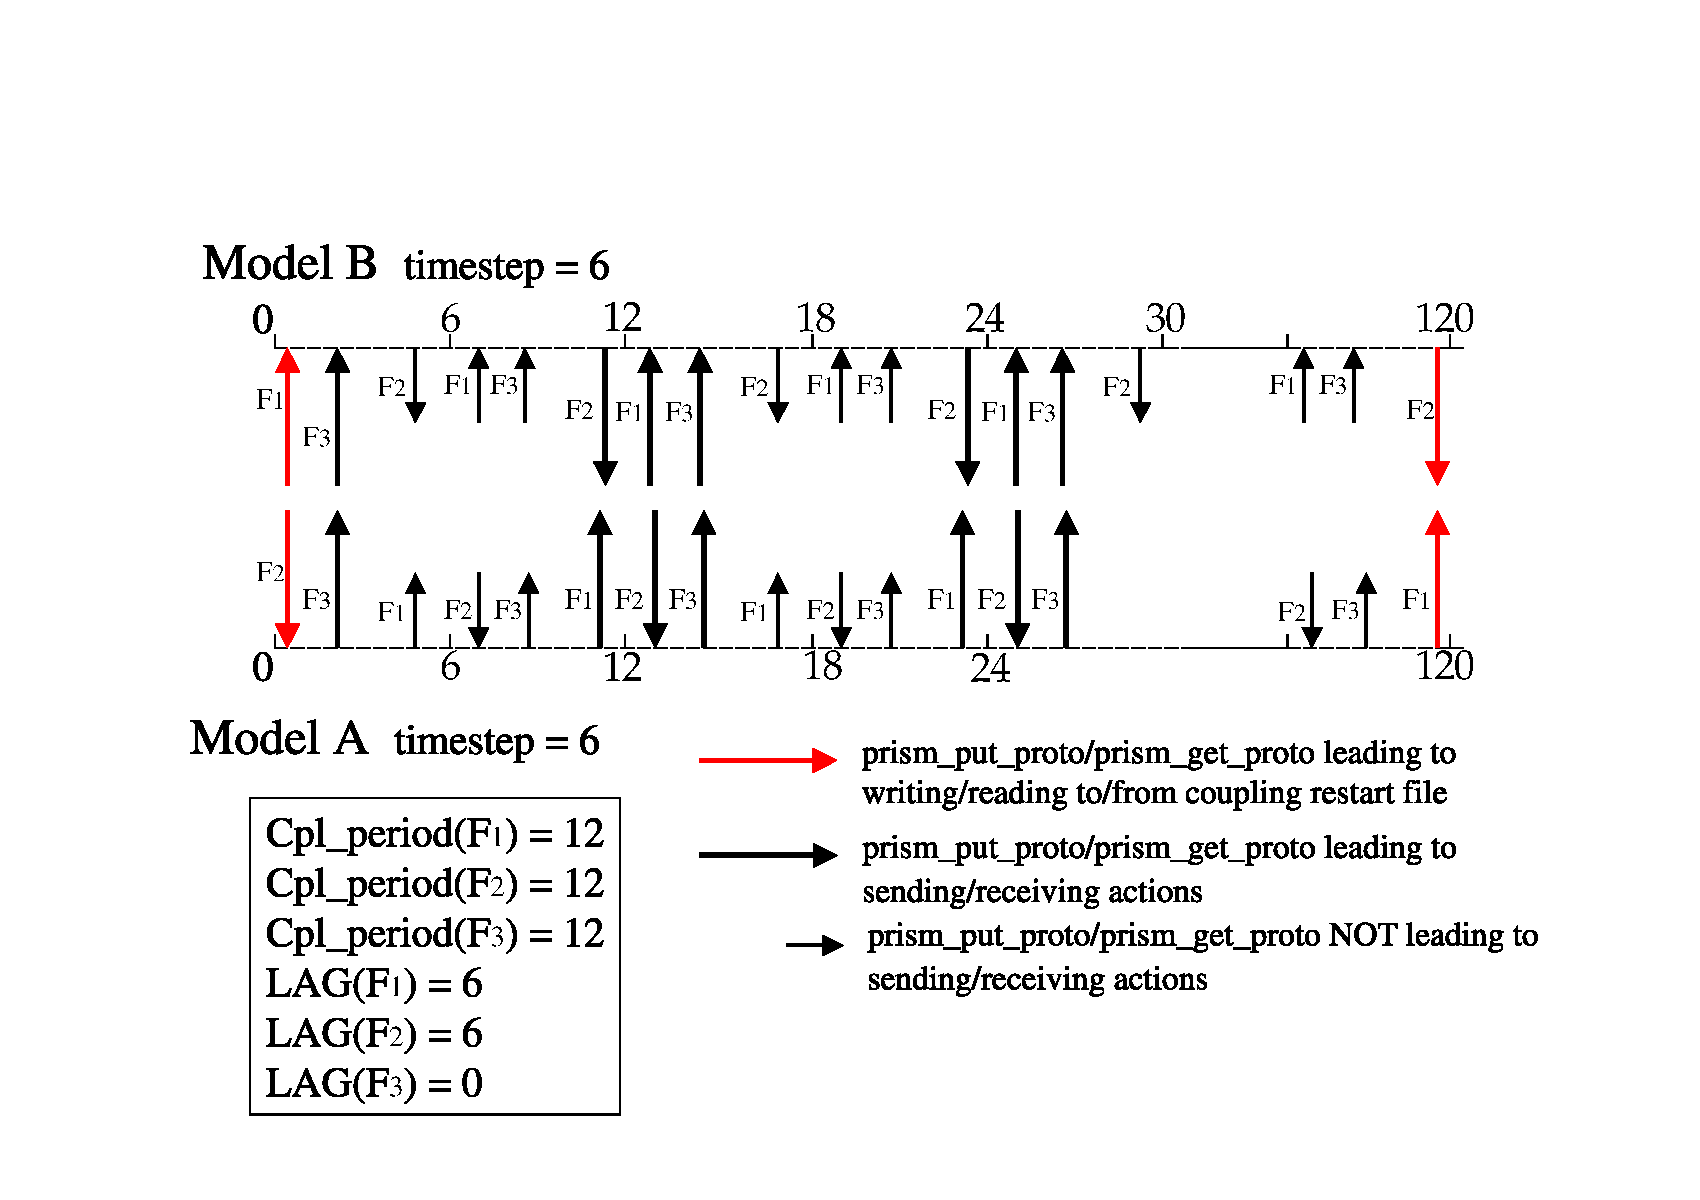
\includegraphics[scale=.6]{figures/fig_lag_concept_2}
    \caption{LAG concept second example}
    \label{fig:lag_concept_2}
  \end{figure}

  For $F_1$ and $F_2$ the situation is similar to the first
  example. Without any lag specified and without any restart file, a deadlock
  would occur as both models would be waiting on a ``get" action. To
  prevent this, $F_1$ and $F_2$ produced at the timestep before have
  to be used to match the model A and model B ``get" actions, which
  means that a lag of 6 must be defined for both $F_1$ and $F_2$. For
  both coupling fields, the {\tt oasis\_put} performed at times 6 and
  18 by the source model then lead to ``put" actions (as 6 + 6 = 12
  and 18 + 6 = 24 which are coupling periods) that match the ``get"
  action performed at time 12 and 24 by the {\tt oasis\_get} called
  by the target model.

  For $F_3$, sent by model A and received by model B, no lag needs to
  be defined: the coupling field produced by model A at the coupling
  timestep can be ``consumed'' by model B without causing a deadlock
  situation.

  As in the first example, the {\tt oasis\_get} performed at the
  beginning of the run for $F_1$ and $F_2$, will automatically receive
  data read from their coupling restart files, and the last {\tt
    oasis\_put} performed at the end of the run automatically write
  them to their coupling restart file. For $F_3$, no coupling restart
  file is needed.

  We see here how the introduction of appropriate LAG indices results
  in receiving in the target component the coupling fields produced by the
  source component the time step before; this is, in some coupling
  configurations, essential to avoid deadlock situations.

\end{enumerate}

\vspace{-0.3cm}
\subsection{The sequence concept}
\label{subsec_sec}

The order of coupling operations in the system is determined solely by
the order of calls to send ({\tt oasis\_put} or ``put'') and receive ({\tt oasis\_get} or ``get'') data in the components
in conjunction with the setting of the lag in the {\it namcouple}.
Data that is received is always blocking while data that is sent is non-blocking with respect to the component making that call.  It
is possible to deadlock the system if the relative orders of puts and
gets in different components are not compatible.

With OASIS3-MCT, the sequence (SEQ) index in the {\it namcouple} file
now provides the coupling layer with an ability to detect a deadlock
before it happens and exit.  It does this by tracking the order of get
and put calls in components compared to the SEQ specified in the {\it
  namcouple}.  If there are any inconsistencies, the component will abort
gracefully with a useable error message before the system deadlocks.
If there are any coupling dependencies in the system, use of the SEQ
index is recommended for diagnosis but has no impact on the ultimate
solution and is NOT required.

In the following two examples, there are two
models, each ``put" a field to the other at every coupling period
without any lags.  In the first case, there is no dependency as each
model first sends and then receives some data.

\begin{verbatim}
     model1        model2
     ------        ------
    put(fld1)     put(fld2)
    get(fld2)     get(fld1)
\end{verbatim}

In this
case, there is no sequencing dependency and the value of SEQ must be
identical (or unset) in the {\it namcouple} description of the fld1
and fld2 coupling.  If by mistake, SEQ is set to 1 for fld1 and 2 for fld2, 
then the coupled model will abort because at runtime, the coupler will
detect in model 2 that fld2 was sent before fld1 was received which
is out of sequence as defined by the SEQ settings.

In the next example, there is a dependency in the sequencing.

\begin{verbatim}
     model1        model2
     ------        ------
    put(fld1)     get(fld1)
                  fld2=g(fld1)
    get(fld2)     put(fld2)
\end{verbatim}

In model2, fld2 depends on fld1. If SEQ is not used and if, for example, model1 does not have the
consistent ordering of the put and get shown above (required by model2), then the models would deadlock and hang. If this dependency is known, there is a benefit in setting SEQ=1 for fld1 and SEQ=2 for fld2; at
runtime, if the sequencing of model1 or model2 does not match the
above diagram, then the  coupling layer will detect it and will exit gracefully with an error message.

Again, the SEQ namecouple setting is only diagnostic and is not
required.



